\documentclass[a4paper,14pt]{extreport}
	\usepackage[left=1.5cm,right=1.5cm,
	    top=1.5cm,bottom=2cm,bindingoffset=0cm]{geometry}
	\usepackage{scrextend}
	\usepackage[T1,T2A]{fontenc}
	\usepackage[utf8]{inputenc}
	\usepackage[english,russian,ukrainian]{babel}
	\usepackage{tabularx}
	\linespread{1.5}
	\usepackage{amssymb}
	\usepackage{fp}
	\usepackage{color}
	\usepackage{amsmath}
	\usepackage{mathrsfs}
	\usepackage{listings}
	\usepackage{graphicx}
	\graphicspath{ {./images/} }
	\usepackage{lipsum}
	\usepackage{xcolor}
	\usepackage{multirow}
	%\usepackage[table,xcdraw]{xcolor}
	\usepackage{hyperref}
	\usepackage{tcolorbox}
	\usepackage{tikz}
	\usepackage[framemethod=TikZ]{mdframed}
	\usepackage{wrapfig,boxedminipage,lipsum}
	\mdfdefinestyle{MyFrame}{%
	linecolor=blue,outerlinewidth=2pt,roundcorner=20pt,innertopmargin=\baselineskip,innerbottommargin=\baselineskip,innerrightmargin=20pt,innerleftmargin=20pt,backgroundcolor=gray!50!white}
	 \usepackage{csvsimple}
	 \usepackage{supertabular}
	\usepackage{pdflscape}
	\usepackage{fancyvrb}
	%\usepackage{comment}
	\definecolor{ggreen}{rgb}{0.4,1,0}
	\definecolor{rred}{rgb}{1,0.1,0.1}
	\definecolor{aquamarine}{rgb}{0.5, 1.0, 0.83}
	\definecolor{amber}{rgb}{1.0, 0.75, 0.0}
	\definecolor{babyblue}{rgb}{0.54, 0.81, 0.94}
	\definecolor{buff}{rgb}{0.94, 0.86, 0.51}
	\definecolor{internationalorange}{rgb}{1.0, 0.31, 0.0}
	\definecolor{lightmauve}{rgb}{0.86, 0.82, 1.0}
	\definecolor{mediumaquamarine}{rgb}{0.4, 0.8, 0.67}
	\usepackage{array,tabularx}
	\usepackage{colortbl}
	
	\usepackage{varwidth}
	\tcbuselibrary{skins}
	\usepackage{fancybox}

	\usetikzlibrary{calc}
	\makeatletter
	\newlength{\mylength}
	\xdef\CircleFactor{1.1}
	\setlength\mylength{\dimexpr\f@size pt}
	\newsavebox{\mybox}
	\newcommand*\circled[2][draw=blue]{\savebox\mybox{\vbox{\vphantom{WL1/}#1}}\setlength\mylength{\dimexpr\CircleFactor\dimexpr\ht\mybox+\dp\mybox\relax\relax}\tikzset{mystyle/.style={circle,#1,minimum height={\mylength}}}
	\tikz[baseline=(char.base)]
	\node[mystyle] (char) {#2};}
	\makeatother
	\usepackage{pgfplots}
    \pgfplotsset{compat=1.9}


	\usepackage{float}
	\usepackage{wrapfig}
	\usepackage{framed}
	%for nice Code{
	\lstdefinestyle{customc}{
	  belowcaptionskip=1\baselineskip,
	  breaklines=true,
	  frame=L,
	  xleftmargin=\parindent,
	  language=C,
	  showstringspaces=false,
	  basicstyle=\small\ttfamily,
	  keywordstyle=\bfseries\color{green!40!black},
	  commentstyle=\itshape\color{purple!40!black},
	  identifierstyle=\color{blue},
	  stringstyle=\color{orange},
	}
	\lstset{escapechar=@,style=customc}
	\usepackage{enumitem}
%}


\begin{document}
\newtcbox{\xmybox}[1][red]{on line, arc=7pt,colback=#1!10!white,colframe=#1!50!black, before upper={\rule[-3pt]{0pt}{10pt}},boxrule=1pt, boxsep=0pt,left=6pt,right=6pt,top=2pt,bottom=2pt}
\pagecolor{white}
\colorlet{Mycolor1}{red!70!orange!700!}



\hyperlink{3v}{37. Широкосмуговий  RC‐підсилювач  на  польовому  транзисторі.  Умова  передачі  сигналу  без 
спотворень. Навести схеми та основні аналітичні вирази для розрахунку схемних функцій.}\\
\hyperlink{4v}{38. Масштабний  неінвертуючий  підсилювач  на  ОП.  Навести  схему  та  основні  співвідношення  для 
розрахунку.}\\
\hyperlink{5v}{39. Масштабний  інвертуючий  підсилювач  на  ОП.  Навести  схему  та  основні  співвідношення  для 
розрахунку.}\\
\hyperlink{6v}{40. Диференціальний  масштабний  підсилювач  на  ОП.  Навести  схему  та  основні  співвідношення  для 
розрахунку.}\\
\hyperlink{7v}{41. Інвертуючий суматор на ОП. Навести схему та основні співвідношення для розрахунку.}\\
\hyperlink{8v}{42.Неінвертуючий суматор на ОП. Навести схему та основні співвідношення для розрахунку}\\
\hyperlink{9v}{43. Диференціальний суматор на ОП. Навести схему та основні співвідношення для розрахунку.}\\
\hyperlink{10v}{44. . Інвертор імпедансу на ОП. Навести схему та основні співвідношення для розрахунку.}\\
\hyperlink{11v}{45.Фазообертач із додатною фазою на ОП. Навести схему та основні співвідношення для розрахунку.}\\
\hyperlink{12v}{46. Фазообертач із від’ємною фазою на ОП. Навести схему та основні співвідношення для розрахунку}\\
\hyperlink{13v}{47. Диференціатор на ОП. Навести схему та основні співвідношення для розрахунку.}\\
\hyperlink{14v}{48. нтегратор на ОП. Навести схему та основні співвідношення для розрахунку}\\
\hyperlink{15v}{49. Початкові умови інтегратора на ОП. Схема скидання інтегратора}\\
\hyperlink{16v}{50. Активний інвертуючий НЧ‐фільтр першого порядку. Навести схему та основні співвідношення для 
розрахунку}\\
\hyperlink{17v}{51.  Активний  неінвертуючий  НЧ‐фільтр  першого  порядку.  Навести  схему  та  основні  співвідношення 
для розрахунку.}\\
\hyperlink{18v}{52. Активний інвертуючий ВЧ‐фільтр першого порядку. Навести схему та основні співвідношення для 
розрахунку.}\\
\hyperlink{19v}{53.Активний  неінвертуючий  ВЧ‐фільтр  першого  порядку.  Навести  схему  та  основні  співвідношення 
для розрахунку.}\\
\hyperlink{20v}{54. Активний  інвертуючий  НЧ‐фільтр  другого  порядку  (схема  Рауха).  Навести  схему  та  основні 
співвідношення для розрахунку.}\\
\hyperlink{21v}{55.  Активний  неінвертуючий  НЧ‐фільтр  другого  порядку  (схема  Саллена‐Кея).  Навести  схему  та 
основні співвідношення для розрахунку.}\\
\hyperlink{22v}{56.  Активний  інвертуючий  ВЧ‐фільтр  другого  порядку  (схема  Рауха).  Навести  схему  та  основні 
співвідношення для розрахунку.}\\
\hyperlink{23v}{57.  Активний неінвертуючий ВЧ‐фільтр другого порядку (схема Саллена‐Кея). Навести схему та основні 
співвідношення для розрахунку. } \\
\hyperlink{24v}{58. Активний  інвертуючий  НЧ‐фільтр  другого  порядку  (схема  Рауха).  Навести  схему  та  основні 
співвідношення для розрахунку.}  \\
\hyperlink{25v}{59. Активний  смуговий  фільтр  другого  порядку  (схема  Саллена‐Кея).  Навести  схему  та  основні 
співвідношення для розрахунку.  }\\
\hyperlink{26v}{60. Активний смуго‐загороджувальний (режекторний) фільтр другого порядку (схема із подвійним Т‐мостом). Навести схему та основні співвідношення для розрахунку}\\
\hyperlink{27v}{61. RС‐генератори із поротом фази у ланцюзі зворотнього зв’язку.}\\
\hyperlink{28v}{62. RС‐генератор з мостом Віна. Навести схему та основні співвідношення для розрахунку}\\
\hyperlink{29v}{63. RС‐генератор з 2Т‐мостом. Навести схему та  основні співвідношення для розрахунку.}\\
\hyperlink{30v}{64.  Загальна характеристика трьохточкових схем LC‐генератора.}\\
\hyperlink{31v}{65. LC‐генератор  з  індуктивною  трьохточкою  в  схемі  СЕ.  Навести  схеми  по  постійному  та  змінному 
струму, основні співвідношення для розрахунку схеми.}\\
\hyperlink{32v}{66. LC‐генератор  з  індуктивною  трьохточкою  в  схемі  СБ.  Навести  схеми  по  постійному  та  змінному 
струму, основні співвідношення для розрахунку схеми }\\
\hyperlink{33v}{67. LC‐генератор  з  індуктивною  трьохточкою  в  схемі  СВ.  Навести  схеми  по  постійному  та  змінному 
струму, основні співвідношення для розрахунку схеми}\\
\hyperlink{34v}{68. LC‐генератор  з  індуктивною  трьохточкою  в  схемі  СЗ.  Навести  схеми  по  постійному  та  змінному 
струму, основні співвідношення для розрахунку схеми}\\
\hyperlink{35v}{69. LC‐генератор  з  ємнісною  трьохточкою  в  схемі  СБ.  Навести  схеми  по  постійному  та  змінному 
струму, основні співвідношення для розрахунку схеми }\\
\hyperlink{36v}{70. LC‐генератор  з  ємнісною  трьохточкою  в  схемі  СБ.  Навести  схеми  по  постійному  та  змінному 
струму, основні співвідношення для розрахунку схеми }\\
\hyperlink{37v}{71. . LC‐генератор  з  ємнісною  трьохточкою  в  схемі  СВ.  Навести  схеми  по  постійному  та  змінному 
струму, основні співвідношення для розрахунку схеми }\\
\hyperlink{38v}{72. LC‐генератор з ємнісною трьохточкою в схемі СЗ. Навести схеми по постійному та змінному струму,
основні співвідношення для розрахунку схеми}\\
\hyperlink{39v}{73. Стабілізація частоти в генераторах гармонічних коливань (кварцовий резонатор)}\\



\newpage 



\begin{landscape}


\hypertarget{3v}{\fbox{37}}\\[1cm]
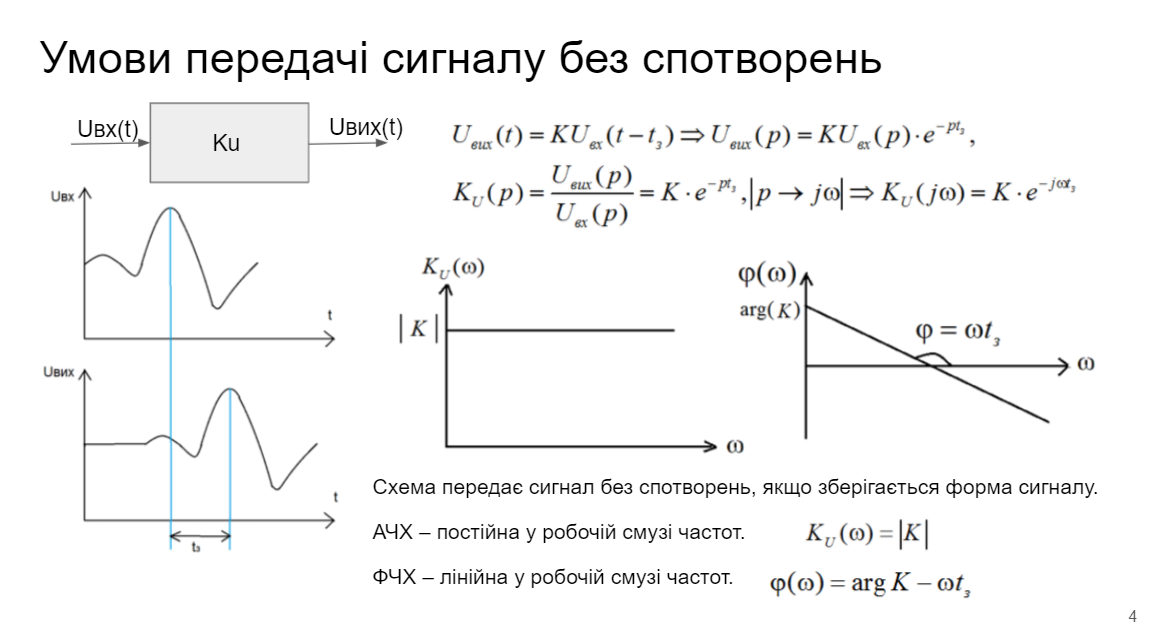
\includegraphics[width=0.5\linewidth]{37.1.png}

\includegraphics[width=0.5\linewidth]{37.2.png}
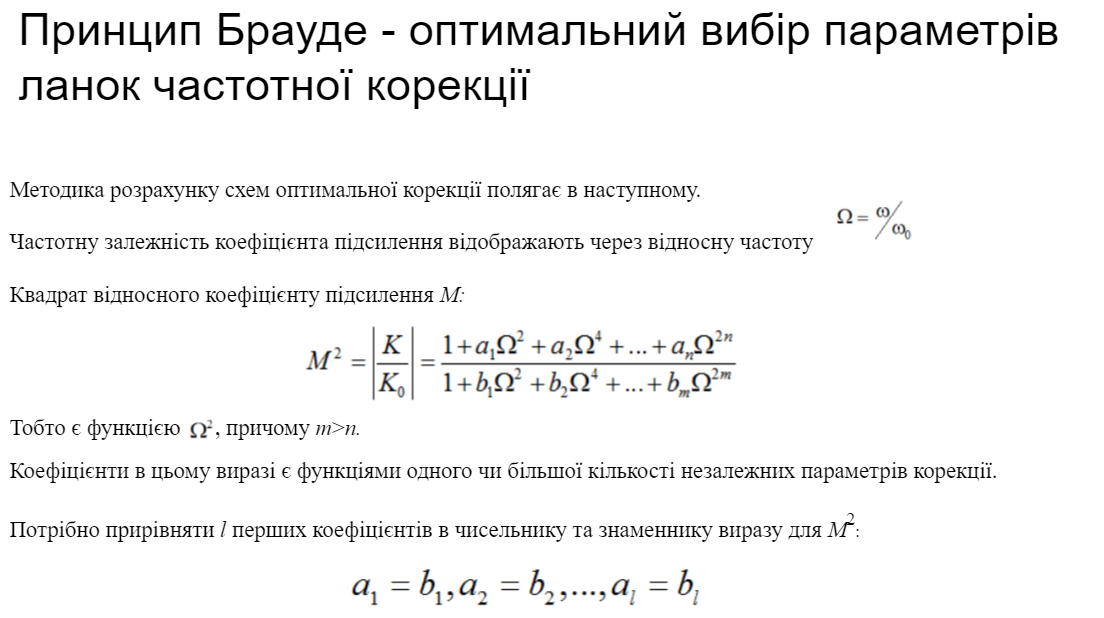
\includegraphics[width=0.6\linewidth]{37.3.png}

\hypertarget{4v}{\fbox{38}}\\[1cm]
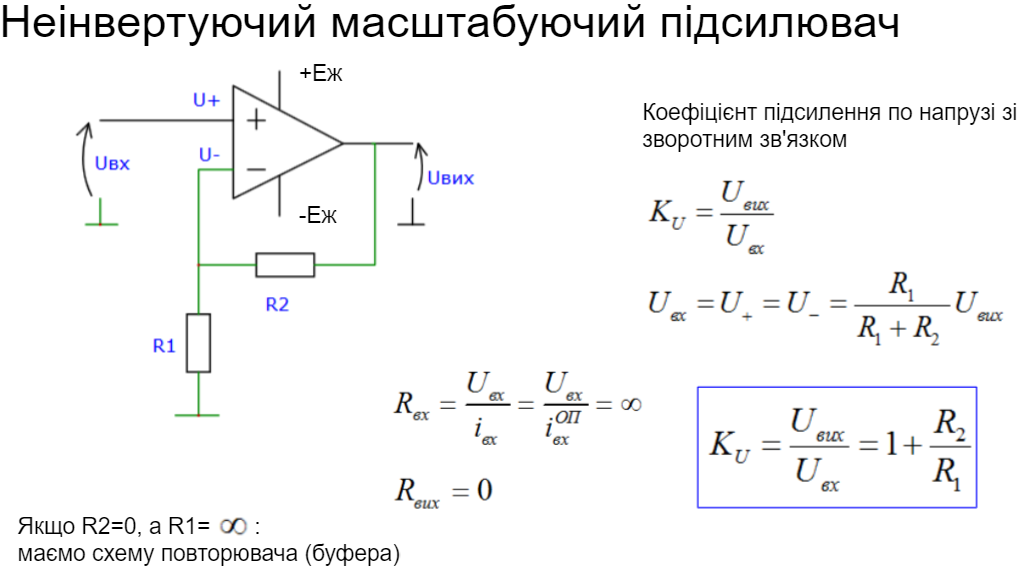
\includegraphics[width=0.45\linewidth]{38.1.png}


\hypertarget{5v}{\fbox{39}}\\[1cm]
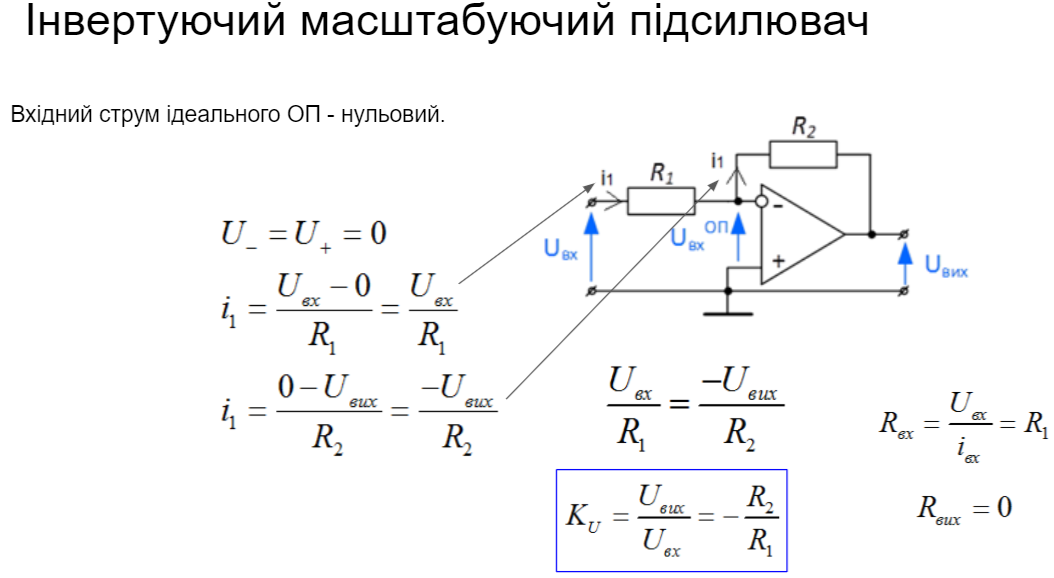
\includegraphics[width=0.5\linewidth]{39.1.png}

\hypertarget{6v}{\fbox{40}}\\[1cm]
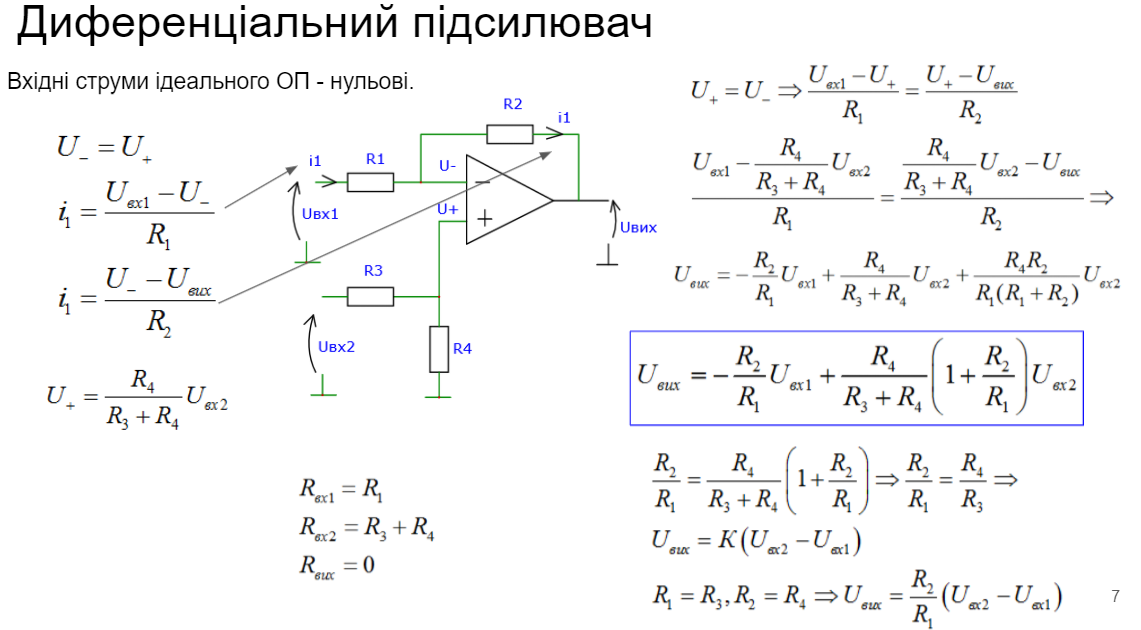
\includegraphics[width=0.5\linewidth]{40.1.png}
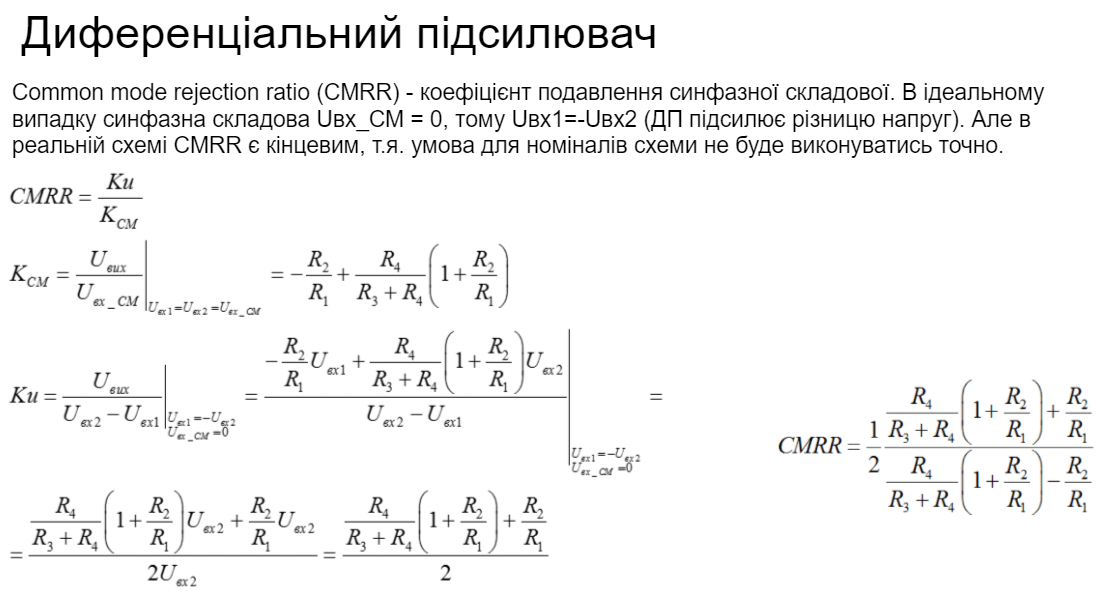
\includegraphics[width=0.5\linewidth]{40.2.png}

\hypertarget{7v}{\fbox{41}}\\[1cm]
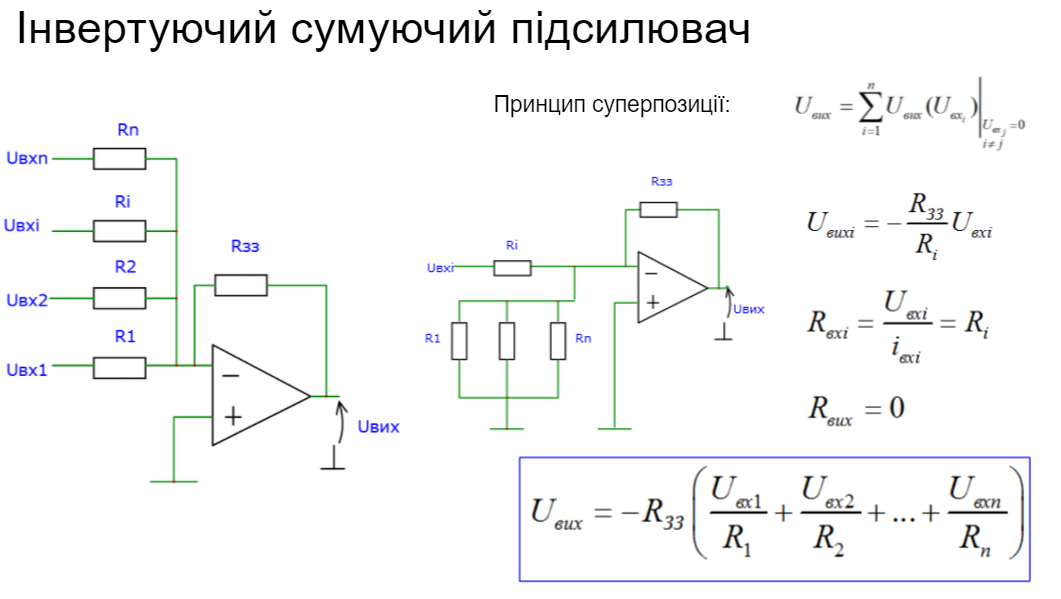
\includegraphics[width=0.45\linewidth]{41.1.png}

\hypertarget{8v}{\fbox{42}}\\[1cm]
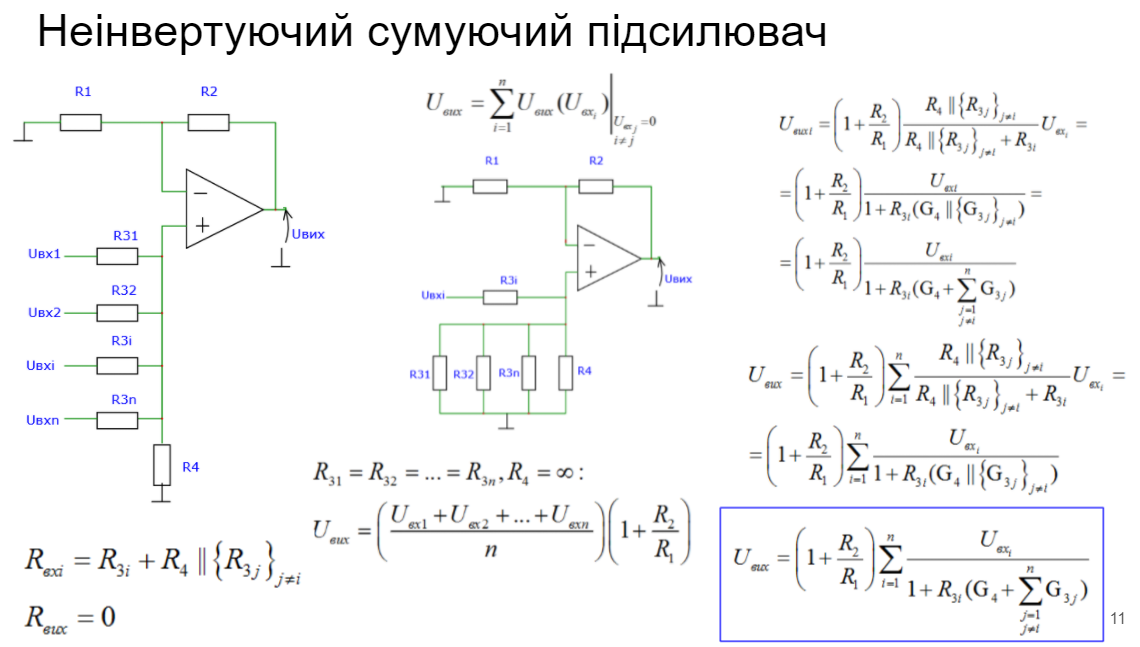
\includegraphics[width=0.5\linewidth]{42.1.png}

\hypertarget{9v}{\fbox{43}}\\[1cm]
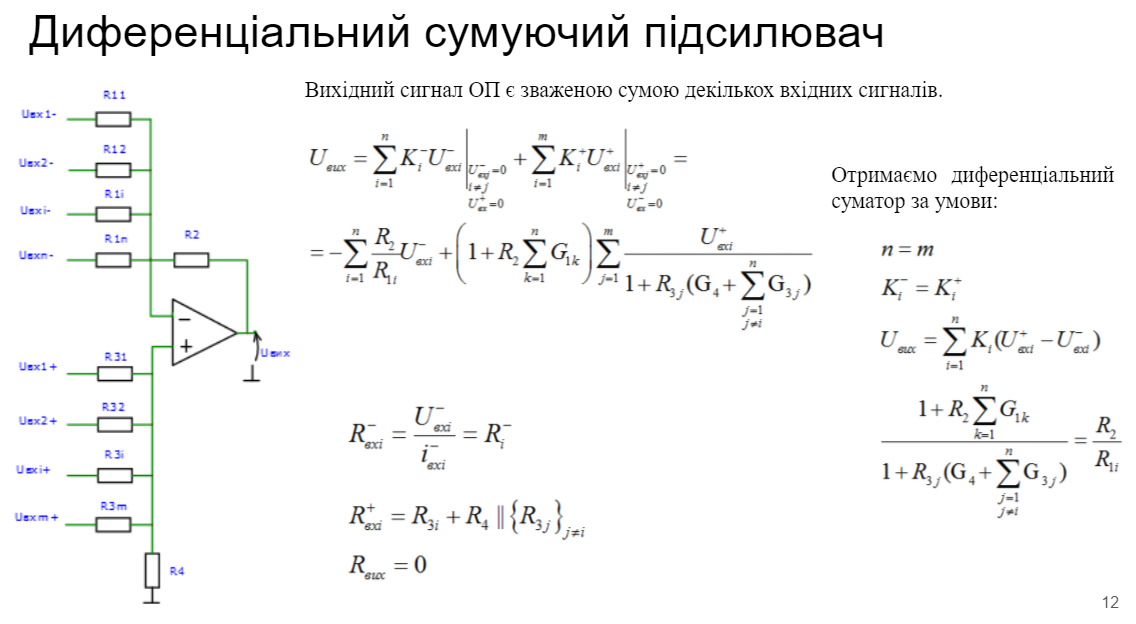
\includegraphics[width=0.45\linewidth]{43.1.png}

\hypertarget{10v}{\fbox{44}}\\[1cm]
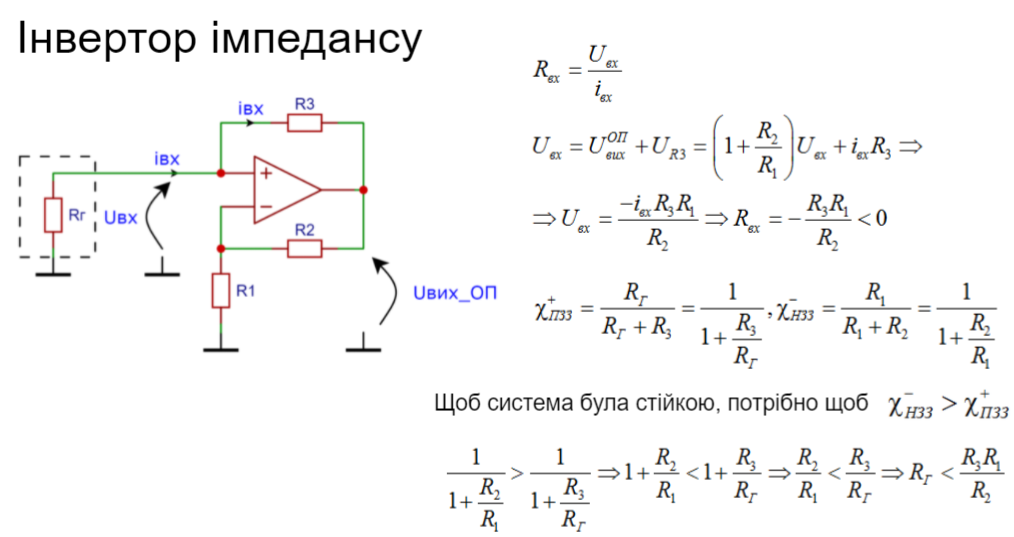
\includegraphics[width=0.5\linewidth]{44.1.png}

\hypertarget{11v}{\fbox{45}}\\[1cm]
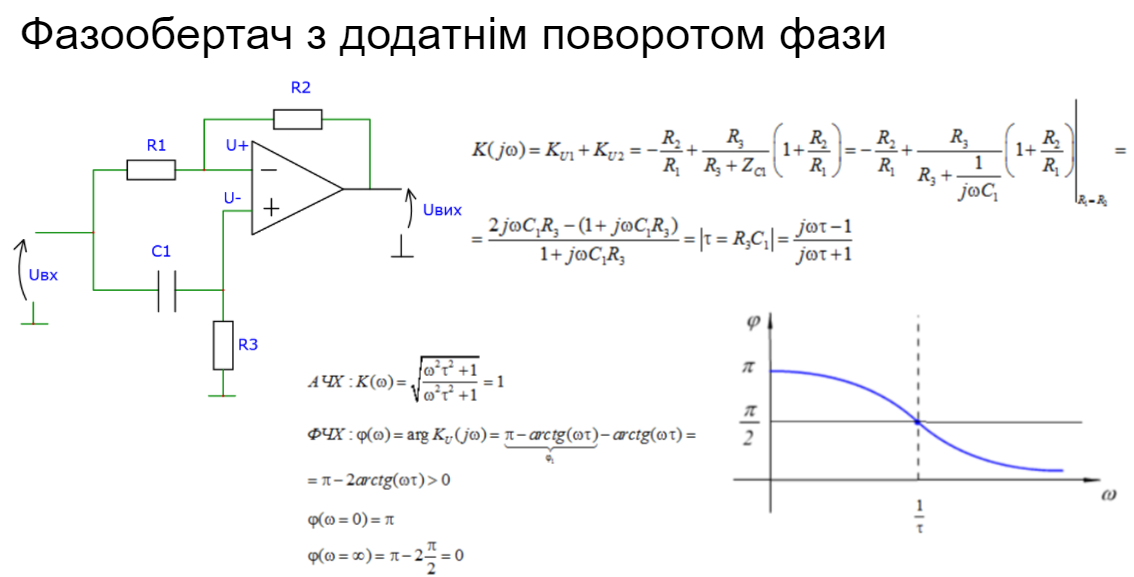
\includegraphics[width=0.5\linewidth]{45.1.png}

\hypertarget{12v}{\fbox{46}}\\[1cm]
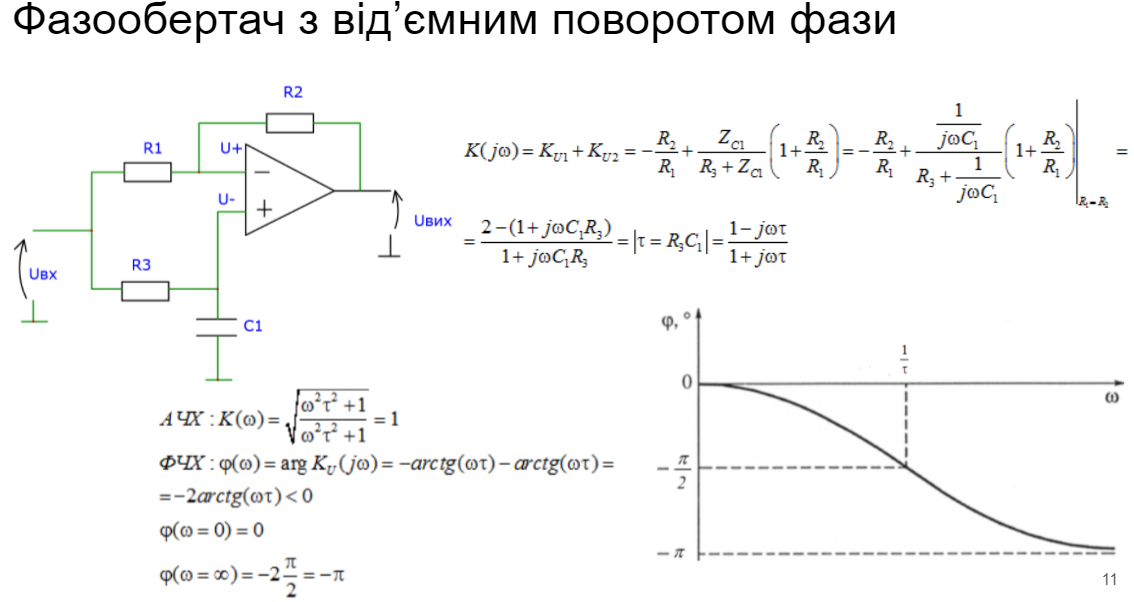
\includegraphics[width=0.5\linewidth]{46.1.png}


\hypertarget{13v}{\fbox{47}}\\[1cm]
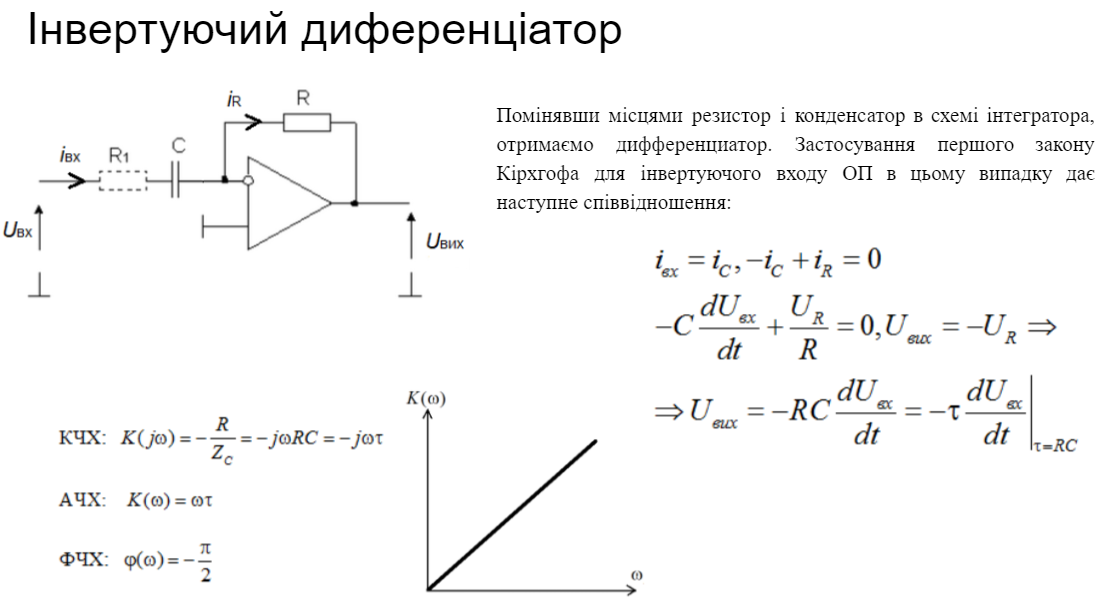
\includegraphics[width=0.5\linewidth]{47.1.png}
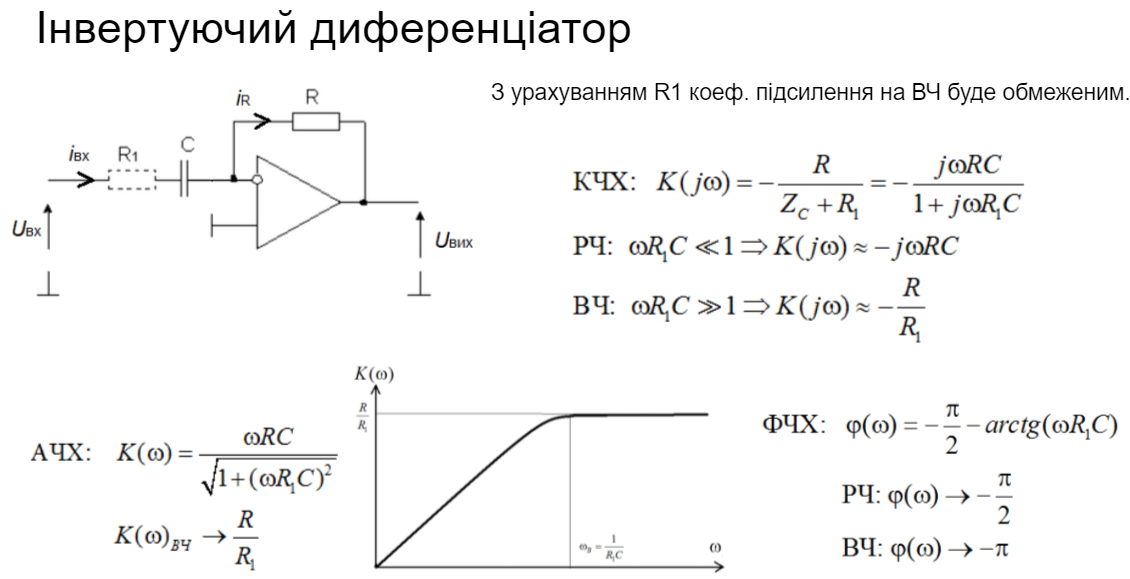
\includegraphics[width=0.5\linewidth]{47.2.png}

\hypertarget{14v}{\fbox{48}}\\[1cm]
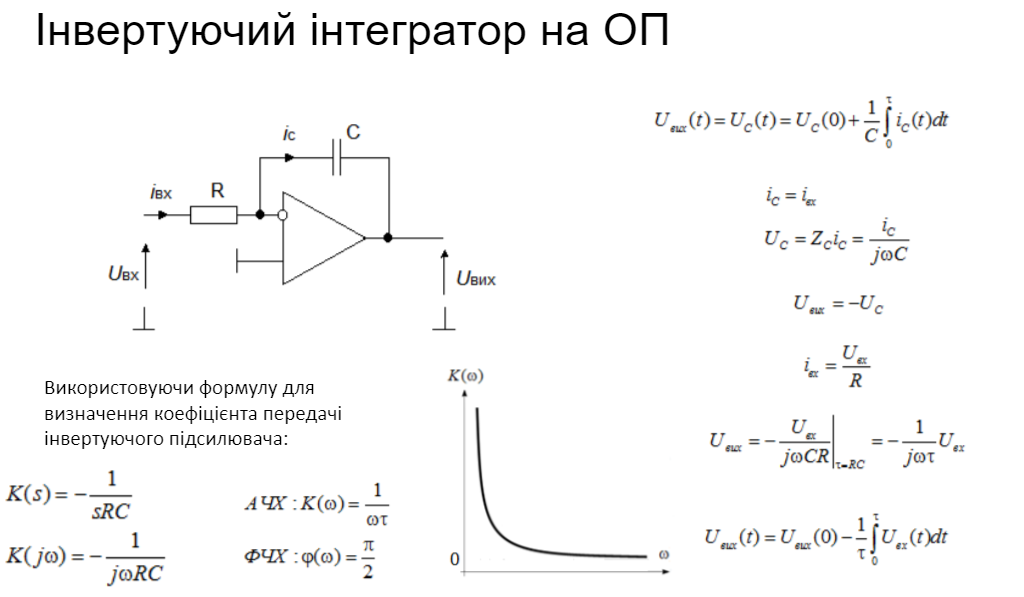
\includegraphics[width=0.5\linewidth]{48.1.png}

\hypertarget{15v}{\fbox{49}}\\[1cm]
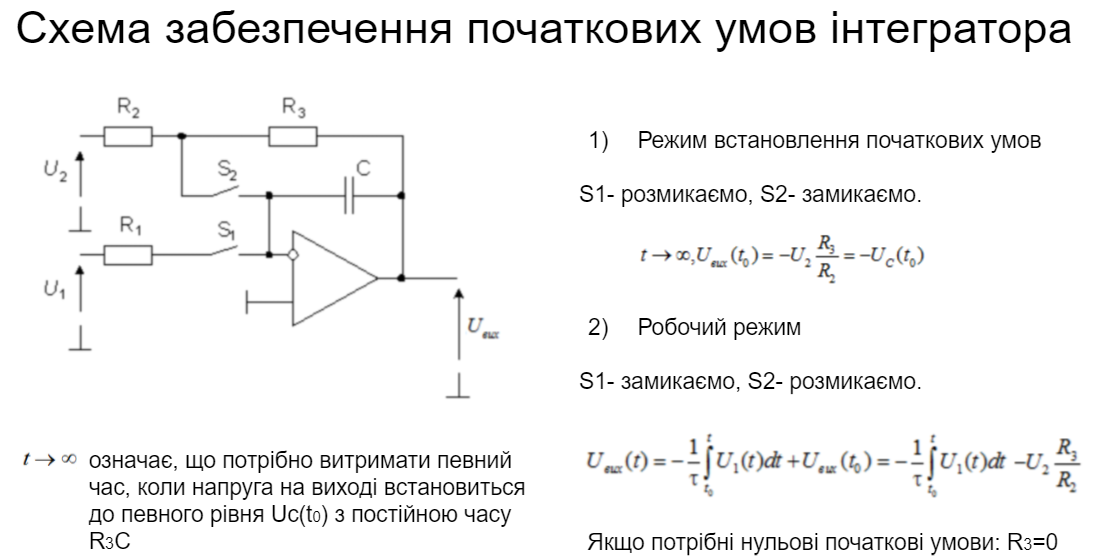
\includegraphics[width=0.5\linewidth]{49.1.png}


\hypertarget{16v}{\fbox{50}}\\[1cm]
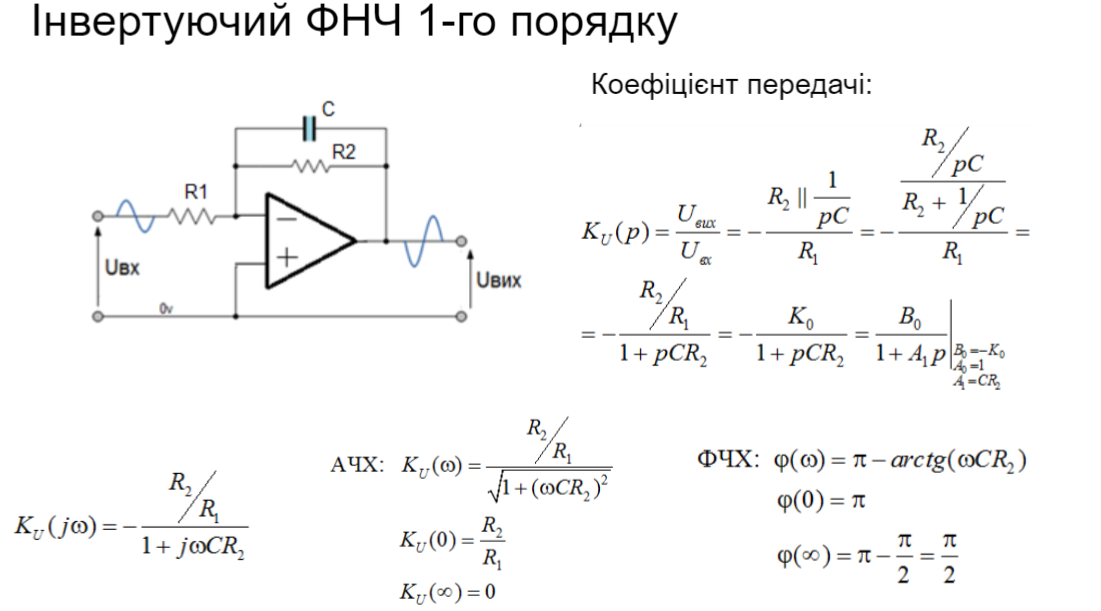
\includegraphics[width=0.5\linewidth]{50.1.png}

\hypertarget{17v}{\fbox{51}}\\[1cm]
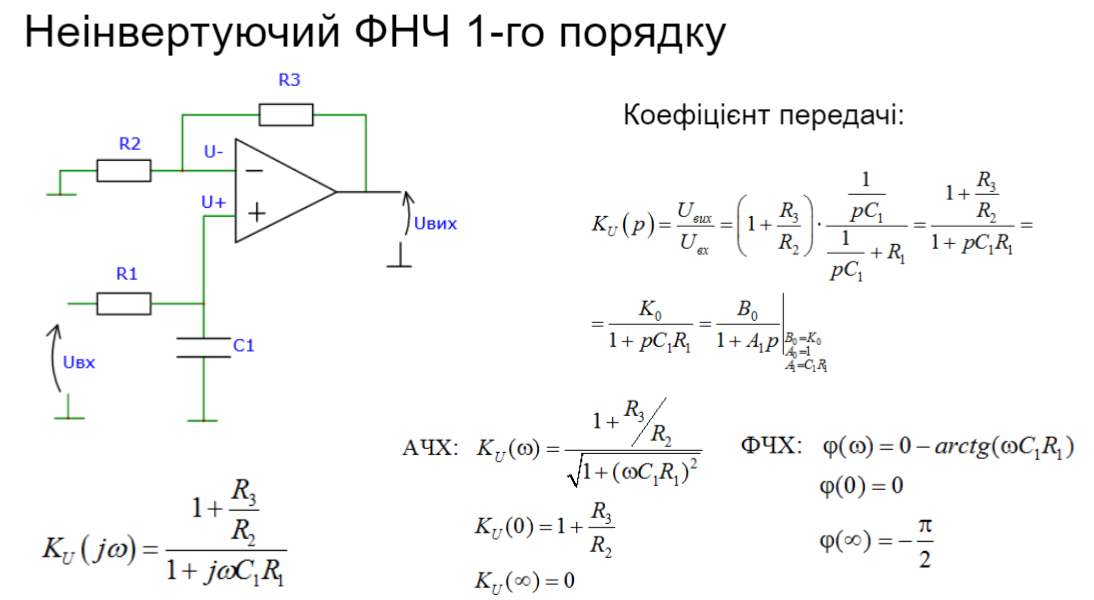
\includegraphics[width=0.45\linewidth]{51.1.png}

\hypertarget{18v}{\fbox{52}}\\[1cm]
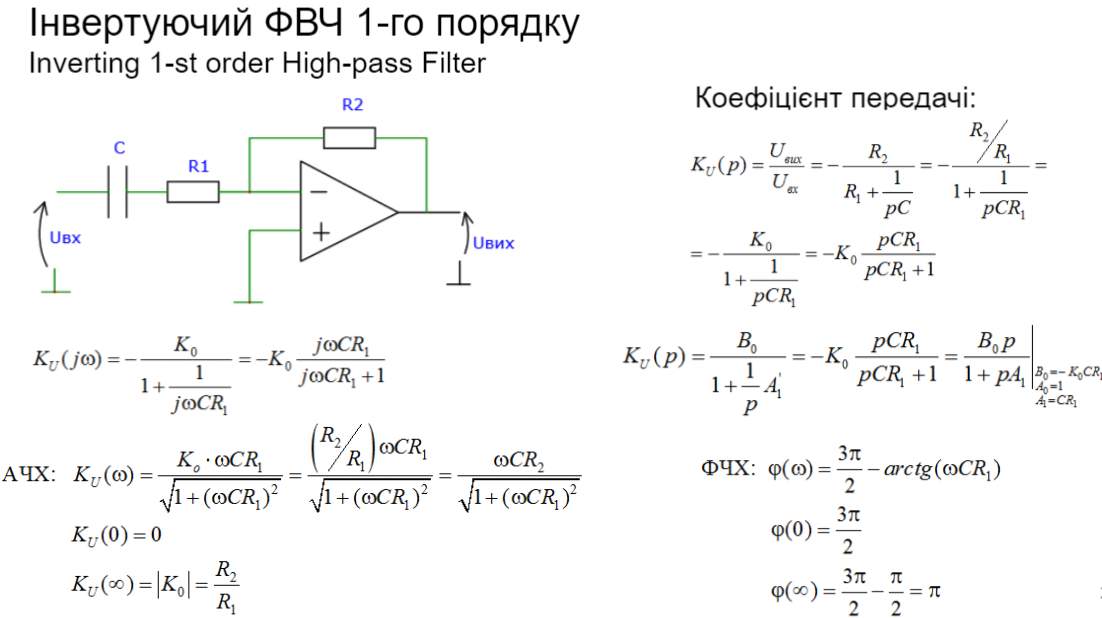
\includegraphics[width=0.5\linewidth]{52.1.png}

\hypertarget{19v}{\fbox{53}}\\[1cm]
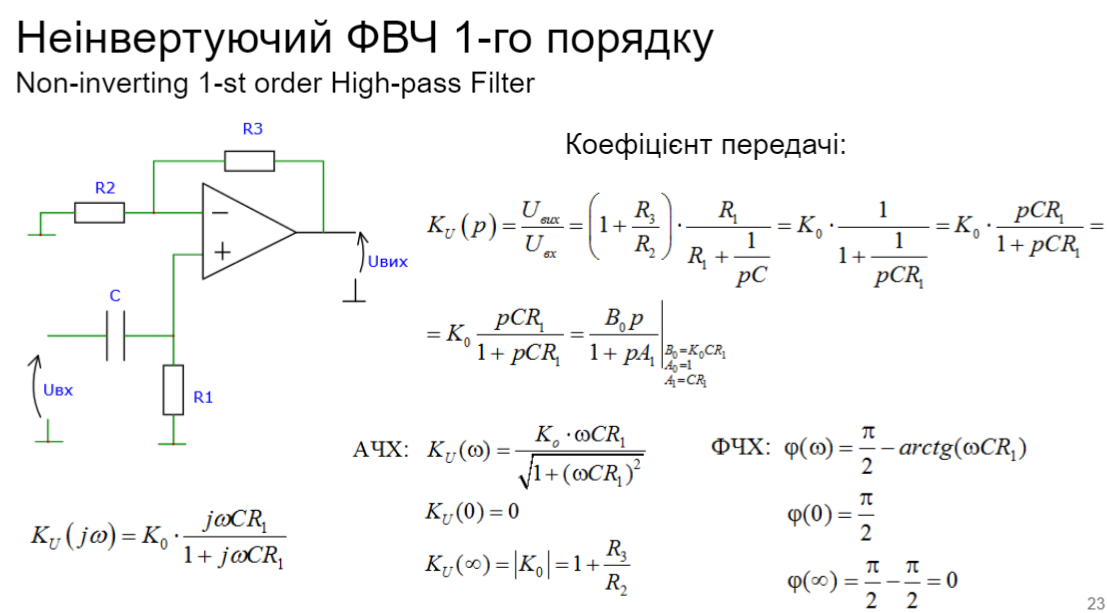
\includegraphics[width=0.45\linewidth]{53.1.png}

\hypertarget{20v}{\fbox{54}}\\[1cm]
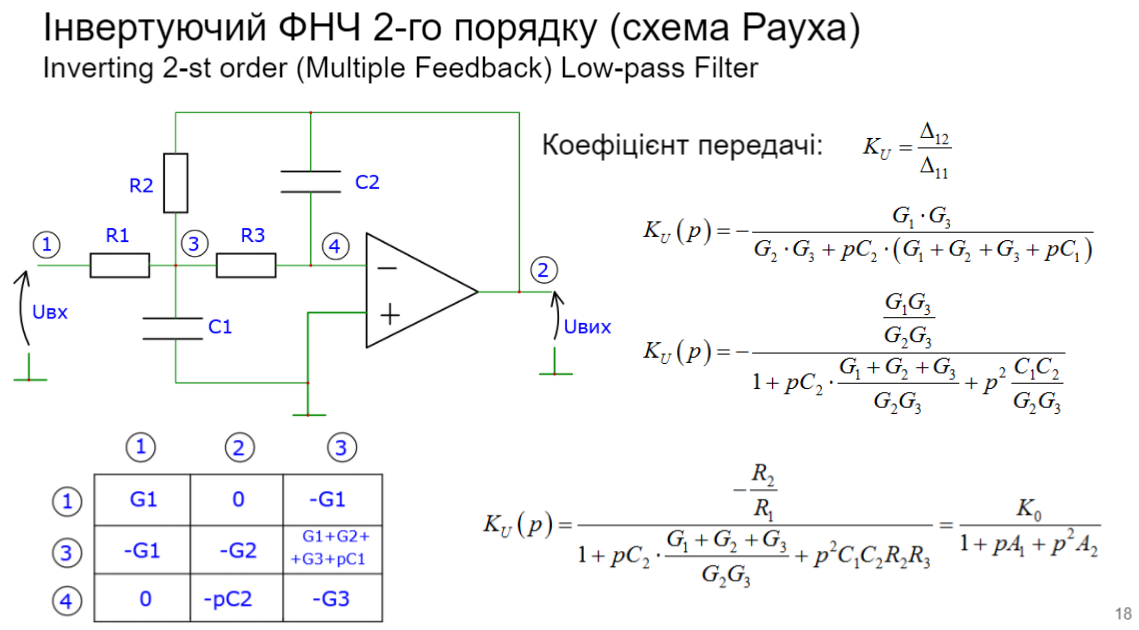
\includegraphics[width=0.5\linewidth]{54.1.png}
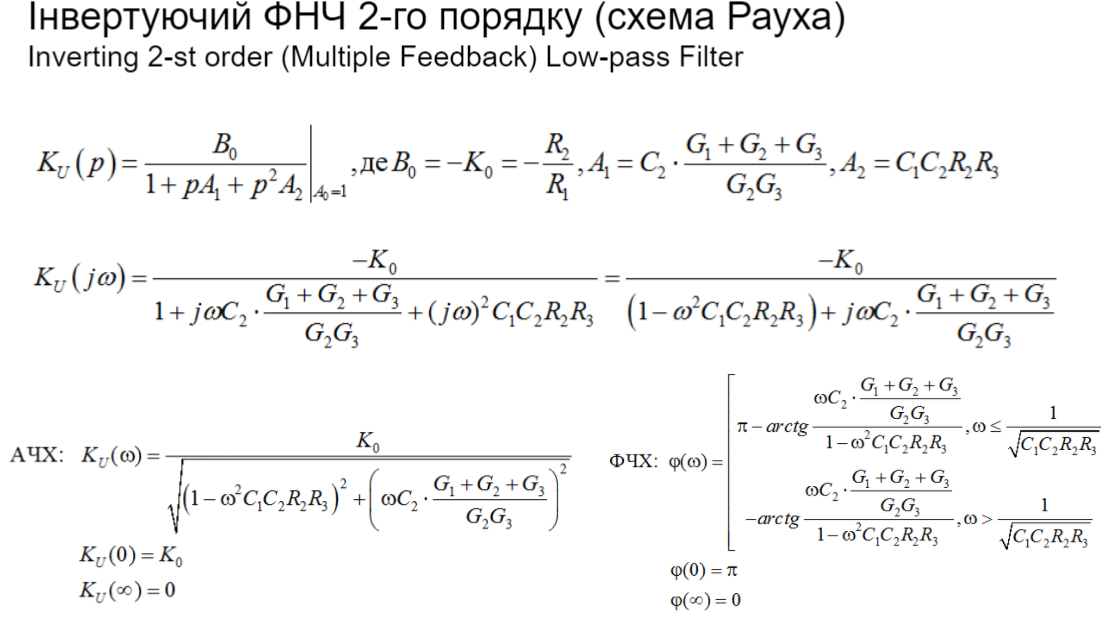
\includegraphics[width=0.5\linewidth]{54.2.png}

\hypertarget{21v}{\fbox{55}}\\[1cm]
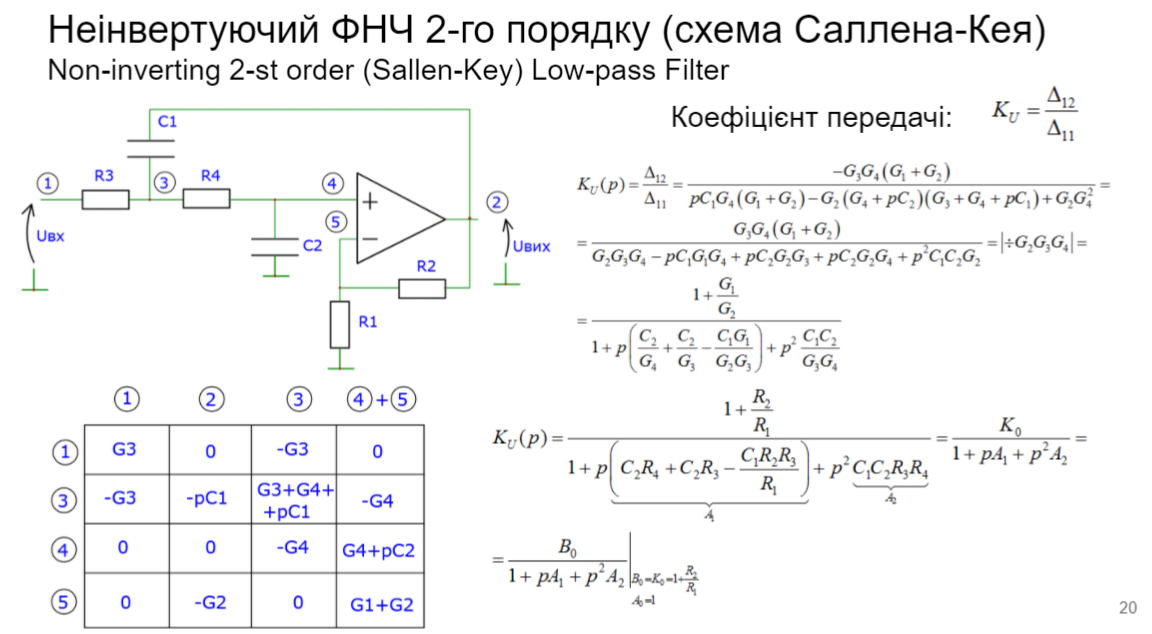
\includegraphics[width=0.45\linewidth]{55.1.png}

\hypertarget{22v}{\fbox{56}}\\
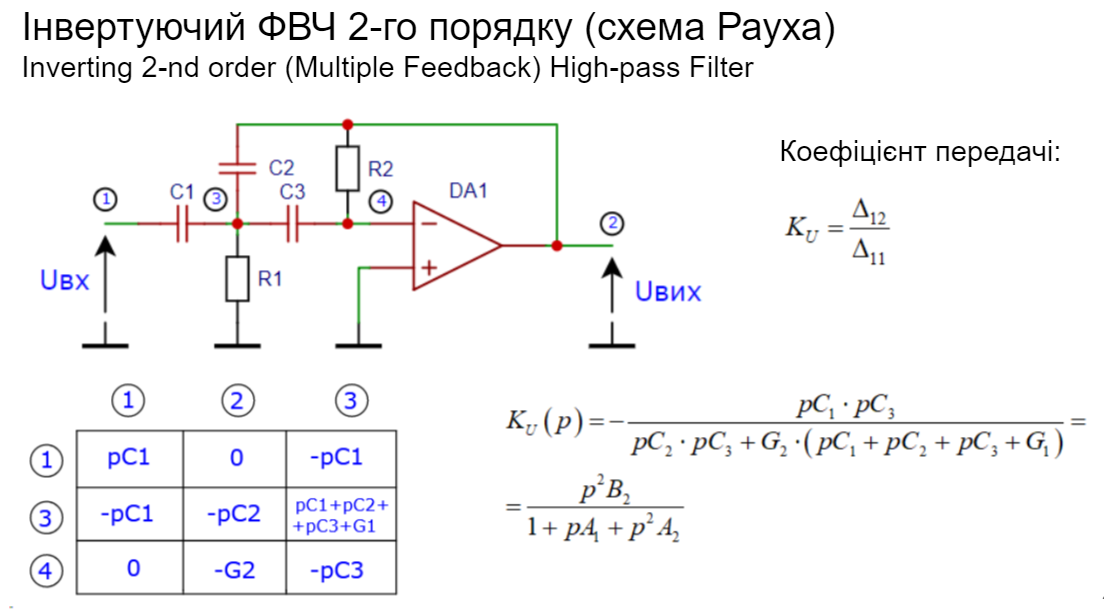
\includegraphics[width=0.5\linewidth]{56.1.png}
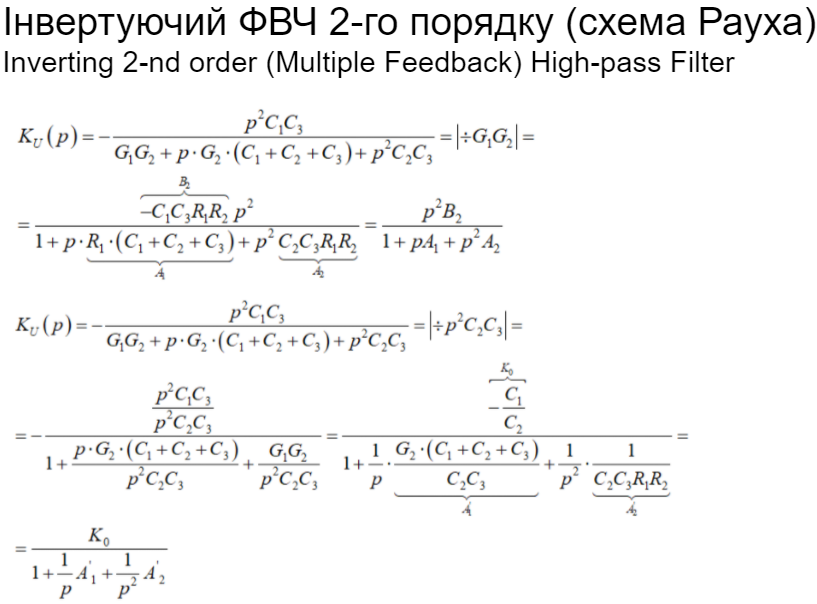
\includegraphics[width=0.5\linewidth]{56.2.png}
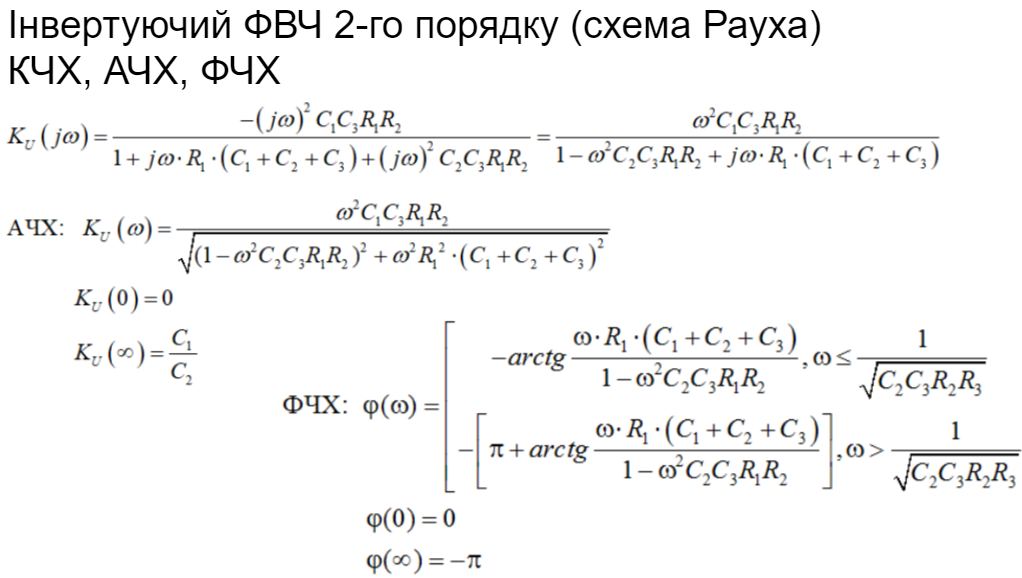
\includegraphics[width=0.5\linewidth]{56.3.png}

\hypertarget{23v}{\fbox{57}}\\[1cm]
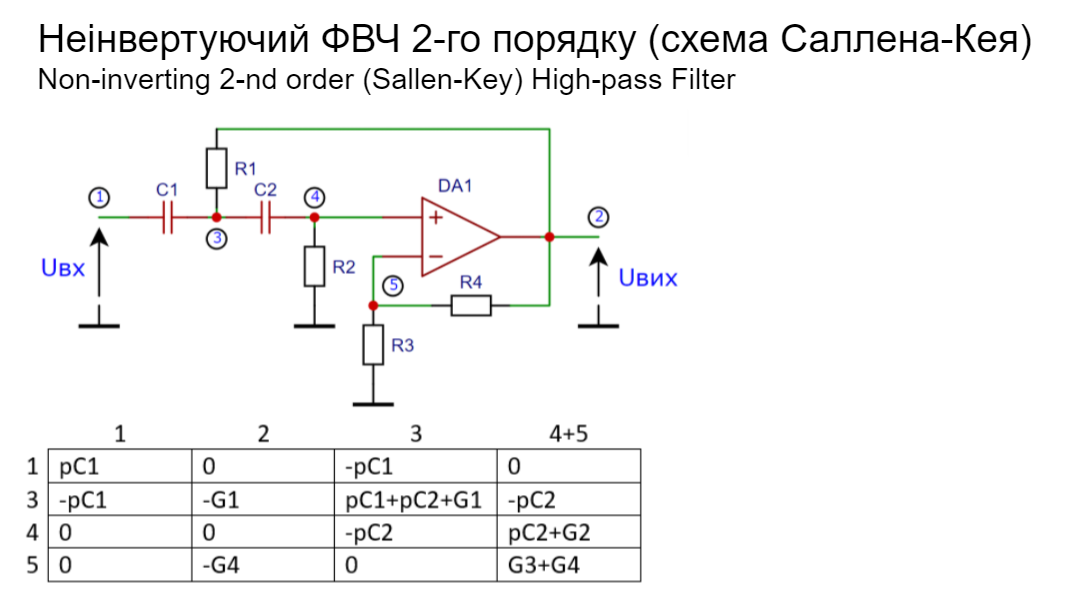
\includegraphics[width=0.5\linewidth]{57.1.png}
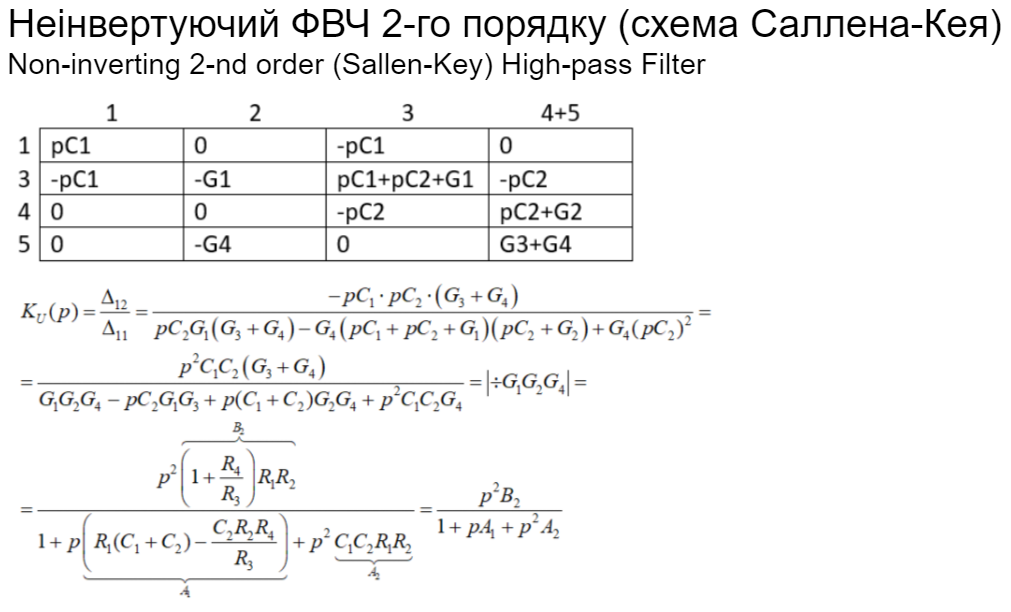
\includegraphics[width=0.5\linewidth]{57.2.png}

\hypertarget{24v}{\fbox{58}}\\[1cm]

\hypertarget{25v}{\fbox{59}}\\[1cm]
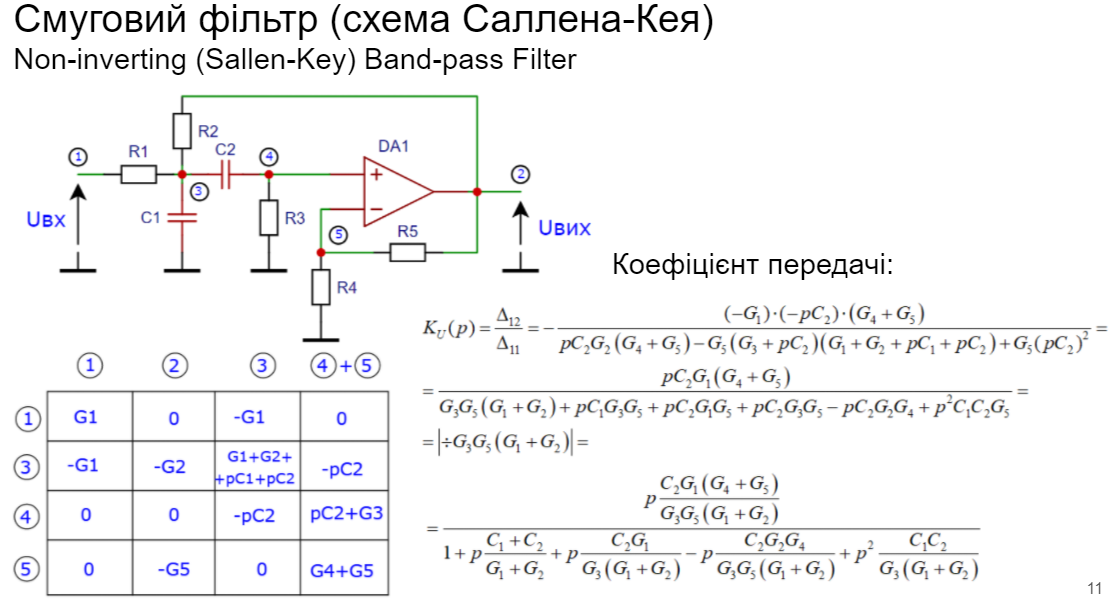
\includegraphics[width=0.5\linewidth]{59.1.png}
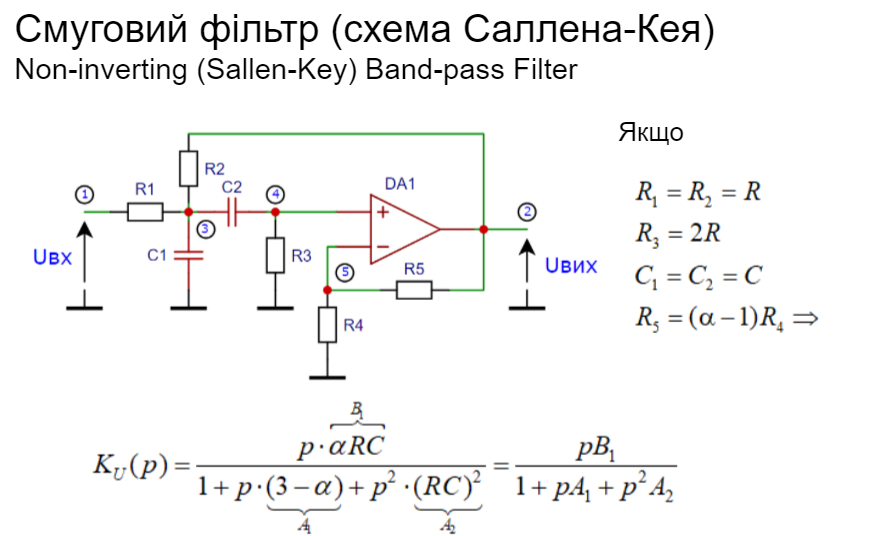
\includegraphics[width=0.5\linewidth]{59.2.png}

\hypertarget{26v}{\fbox{60}}\\[1cm]
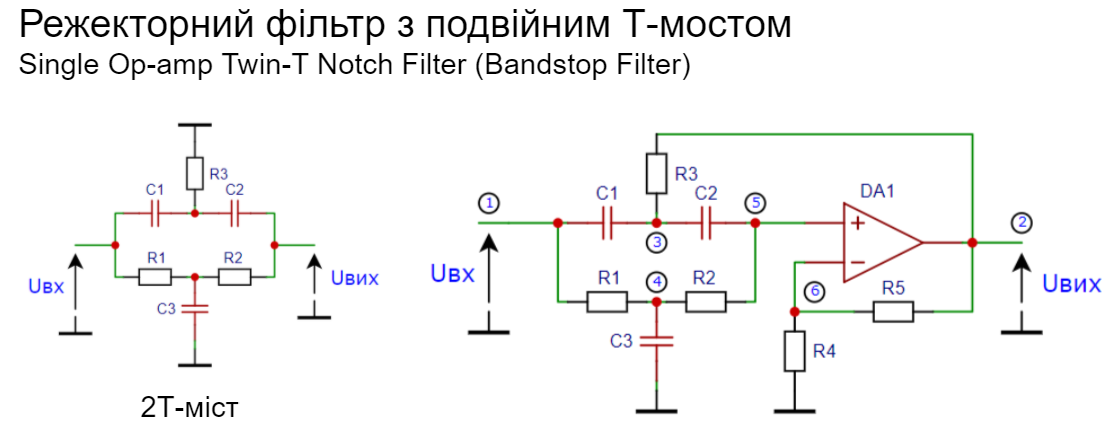
\includegraphics[width=0.5\linewidth]{60.1.png}
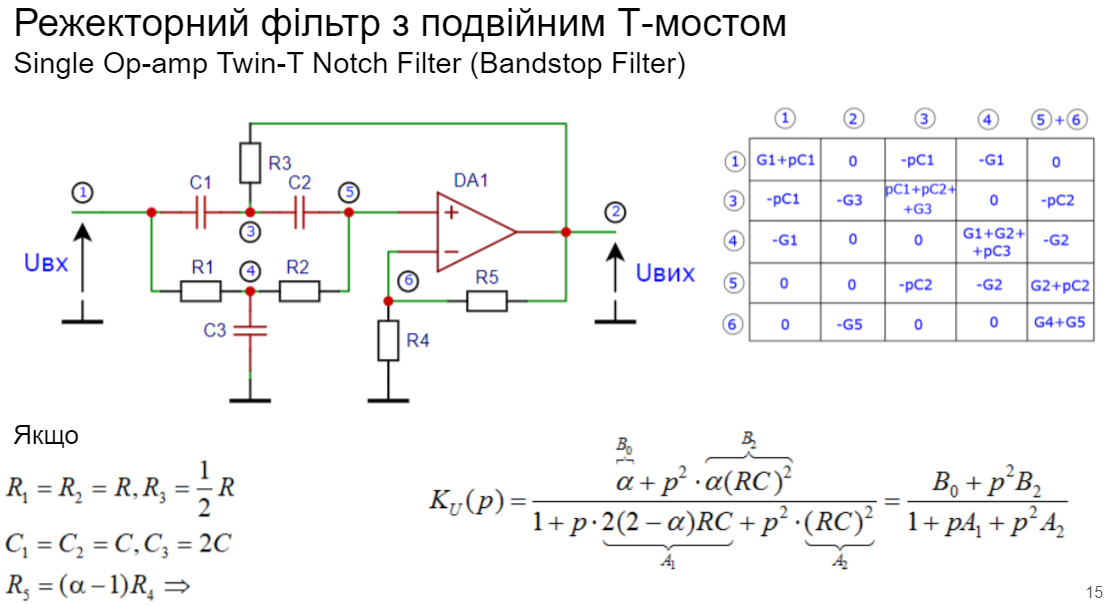
\includegraphics[width=0.5\linewidth]{60.2.png}

\hypertarget{27v}{\fbox{61}}\\[1cm]
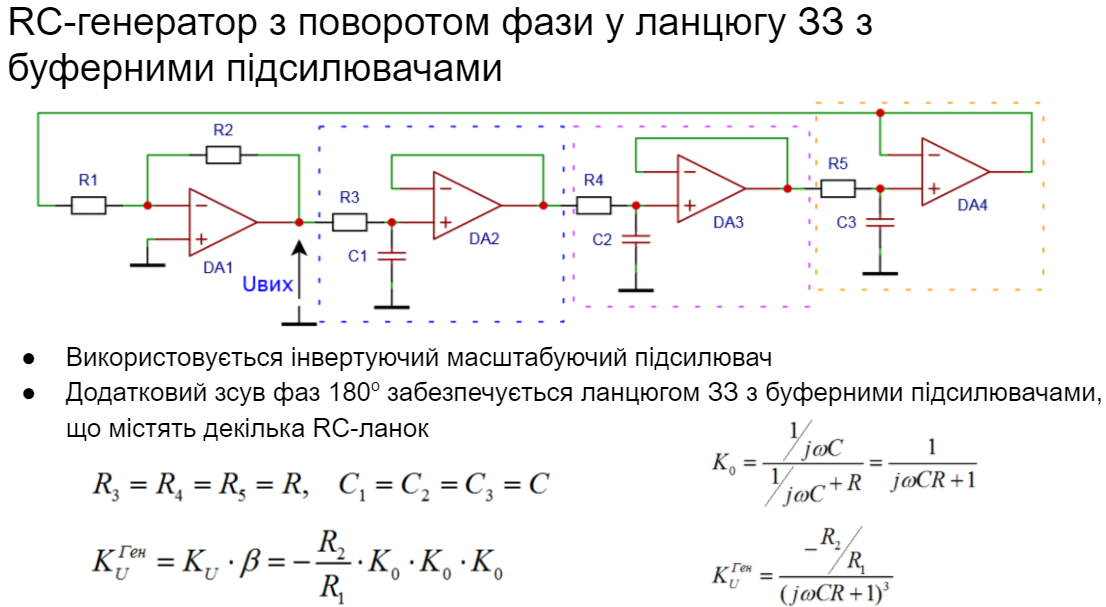
\includegraphics[width=0.5\linewidth]{61.1.png}
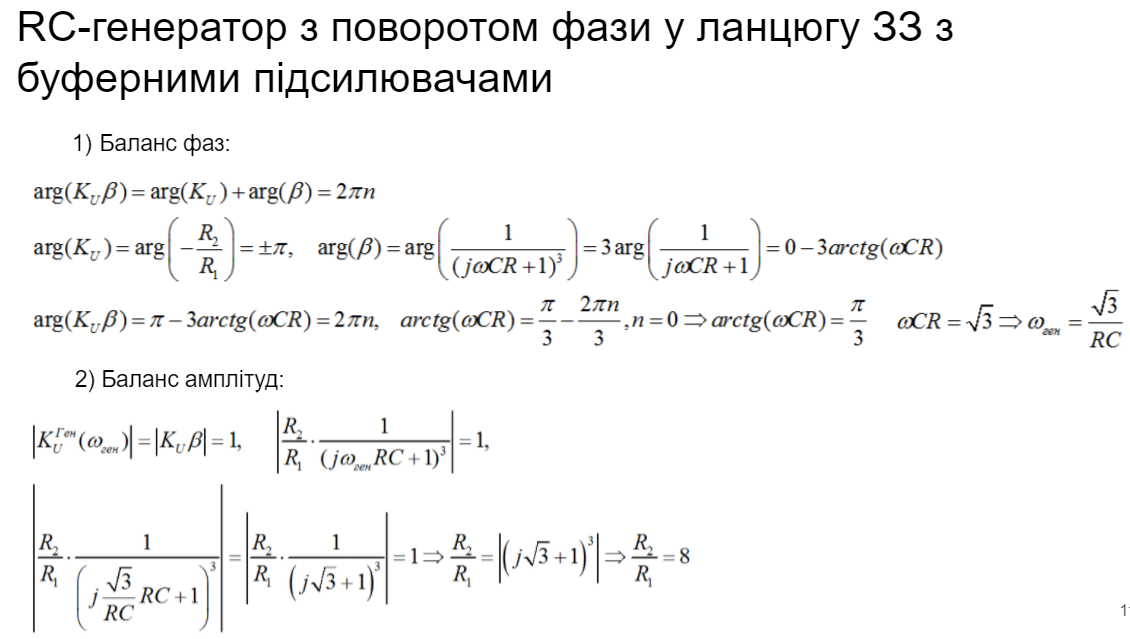
\includegraphics[width=0.5\linewidth]{61.2.png}

\hypertarget{28v}{\fbox{62}}\\[1cm]
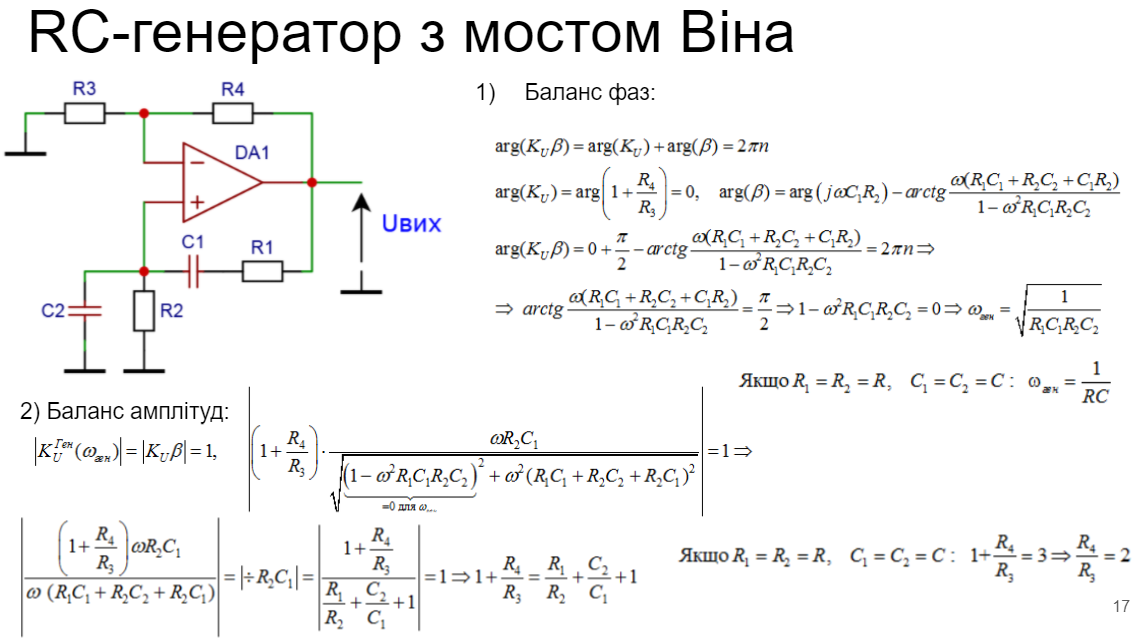
\includegraphics[width=0.45\linewidth]{62.1.png}

\hypertarget{29v}{\fbox{63}}\\[1cm]
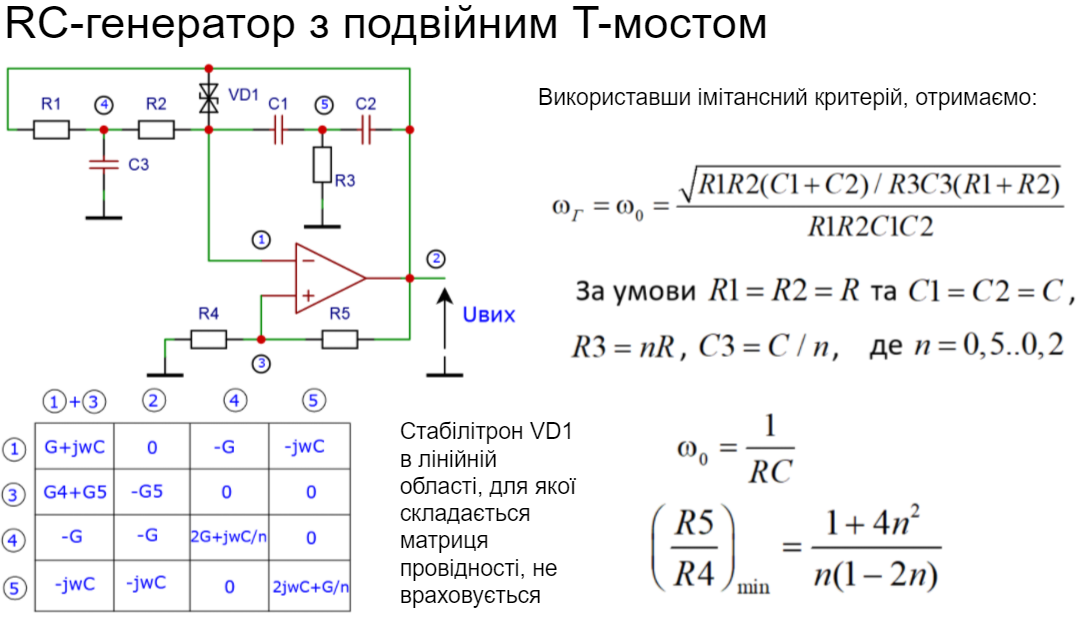
\includegraphics[width=0.5\linewidth]{63.1.png}

\hypertarget{30v}{\fbox{64}}\\[1cm]
neeby
\newpage
\hypertarget{31v}{\fbox{65}}\\[1cm]
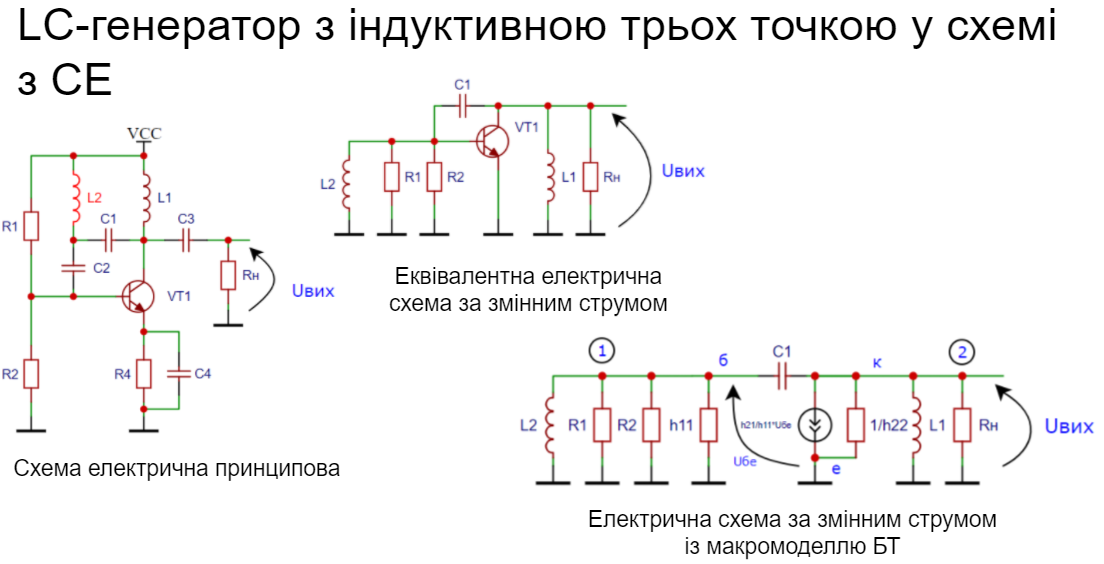
\includegraphics[width=0.5\linewidth]{65.1.png}
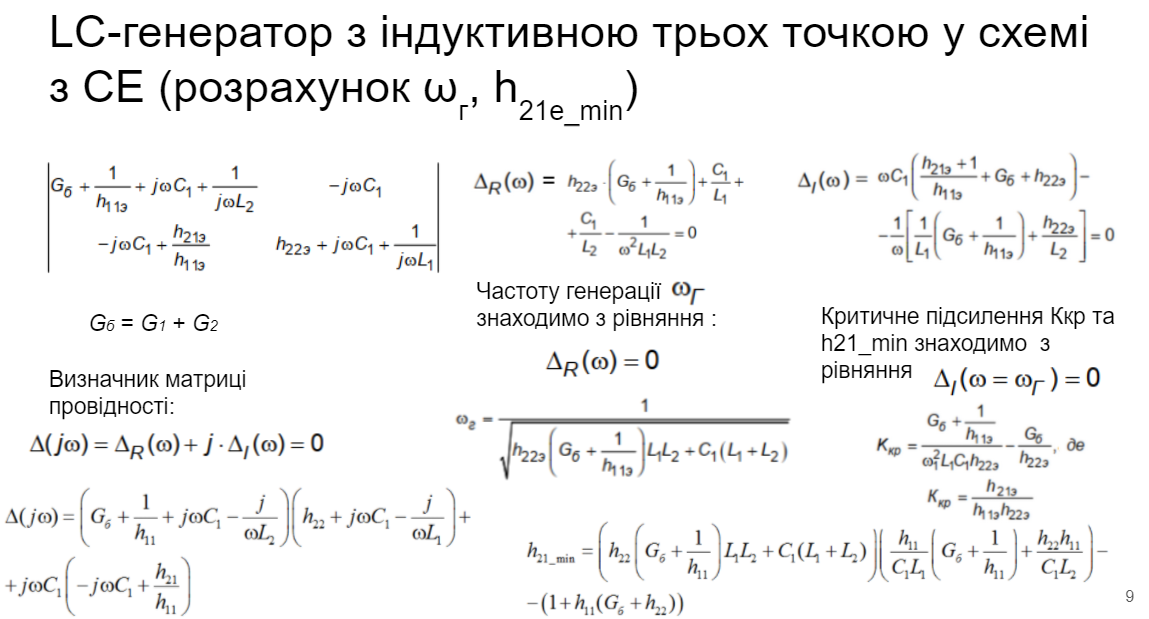
\includegraphics[width=0.5\linewidth]{65.2.png}

\hypertarget{32v}{\fbox{66}}\\[1cm]
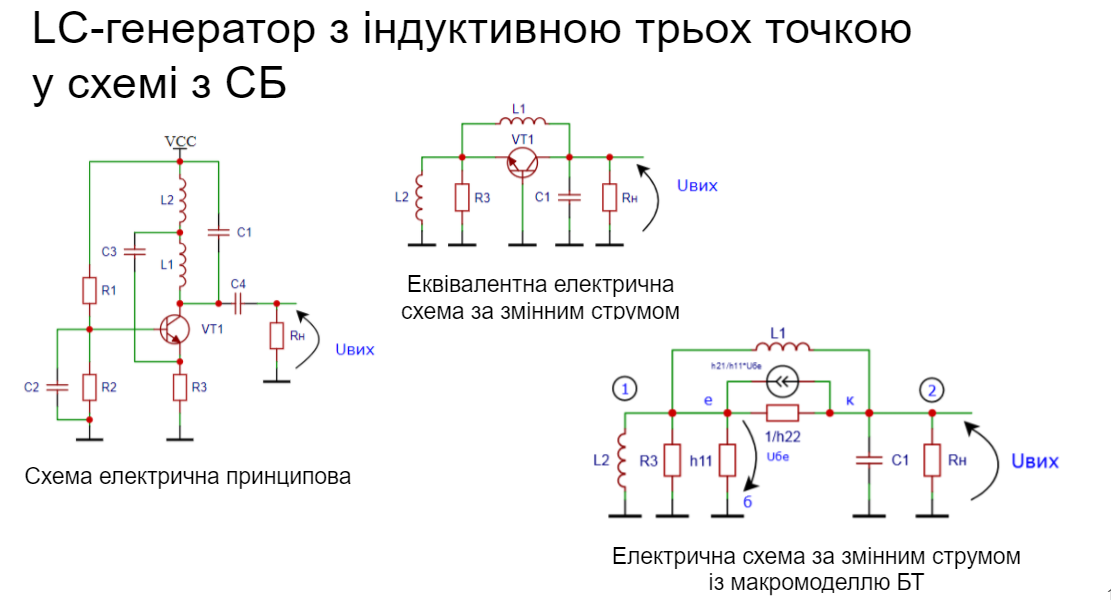
\includegraphics[width=0.5\linewidth]{66.1.png}
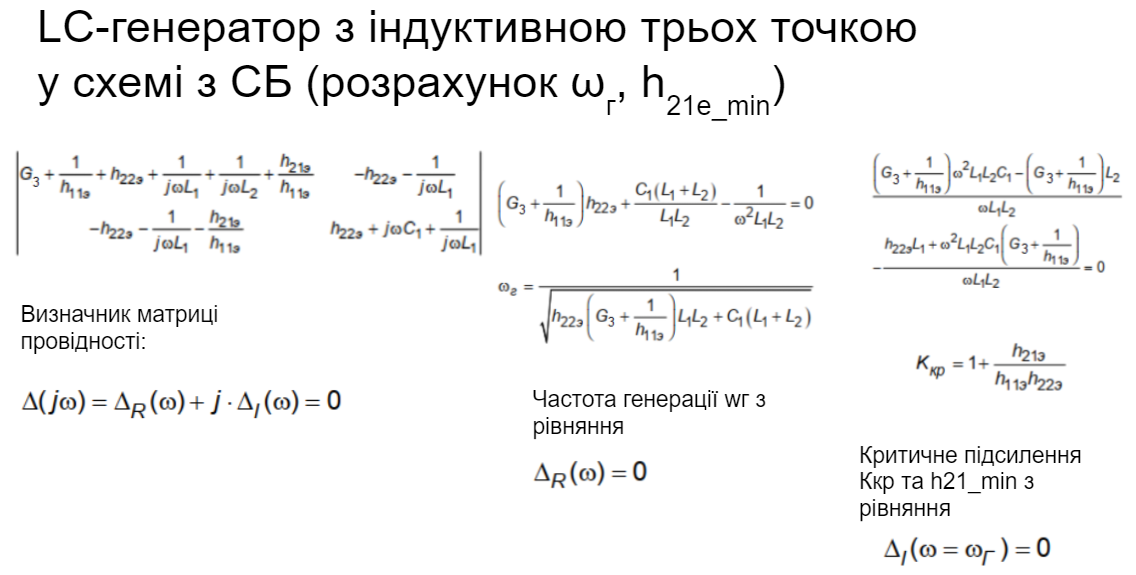
\includegraphics[width=0.5\linewidth]{66.2.png}

\hypertarget{33v}{\fbox{67}}\\[1cm]
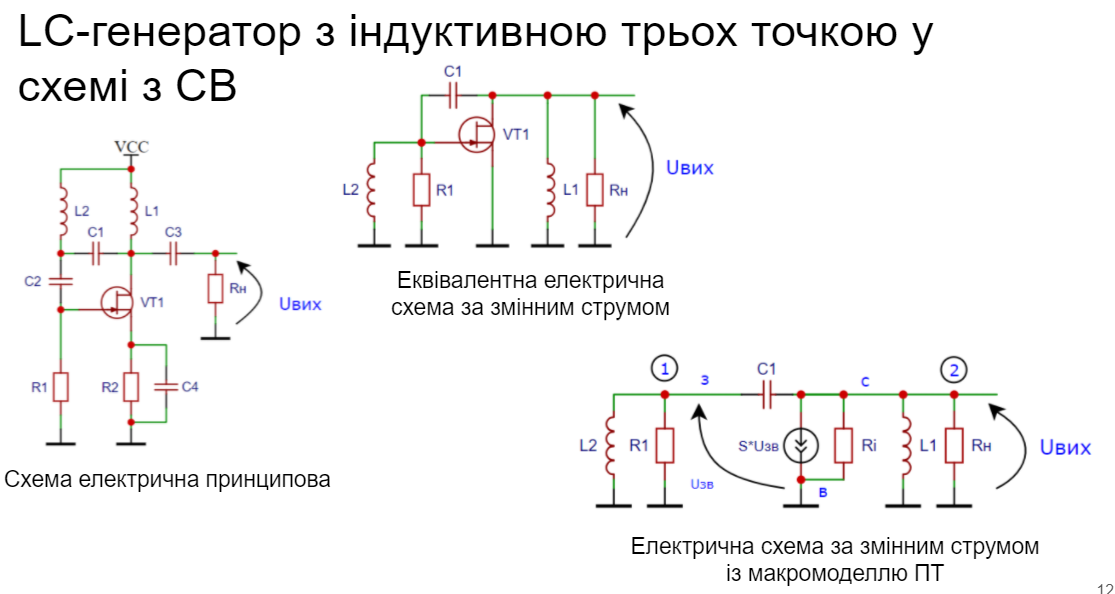
\includegraphics[width=0.5\linewidth]{67.1.png}
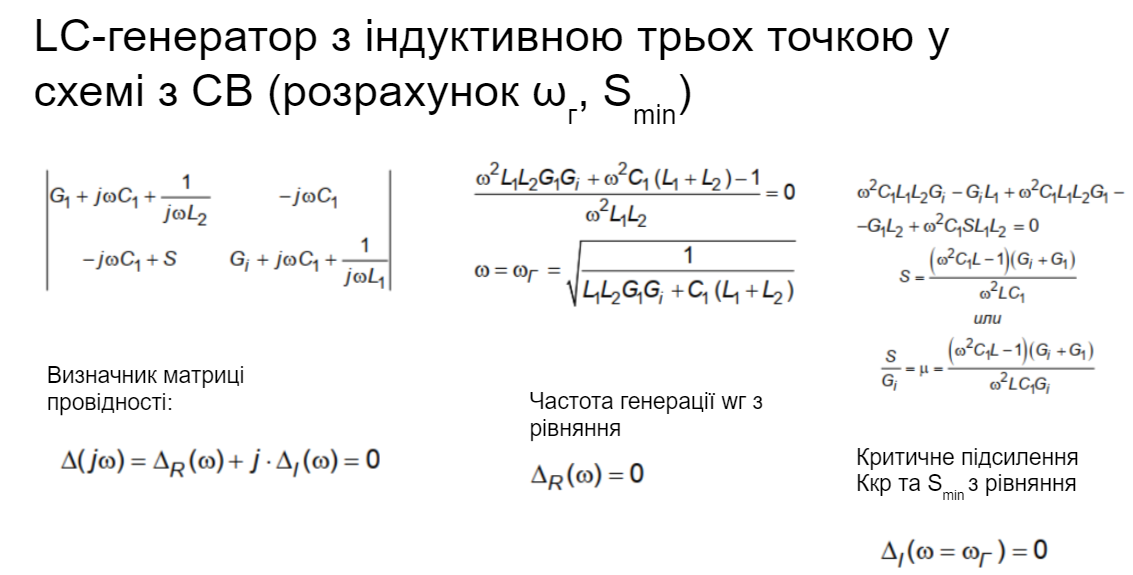
\includegraphics[width=0.5\linewidth]{67.2.png}

\hypertarget{34v}{\fbox{68}}\\[1cm]
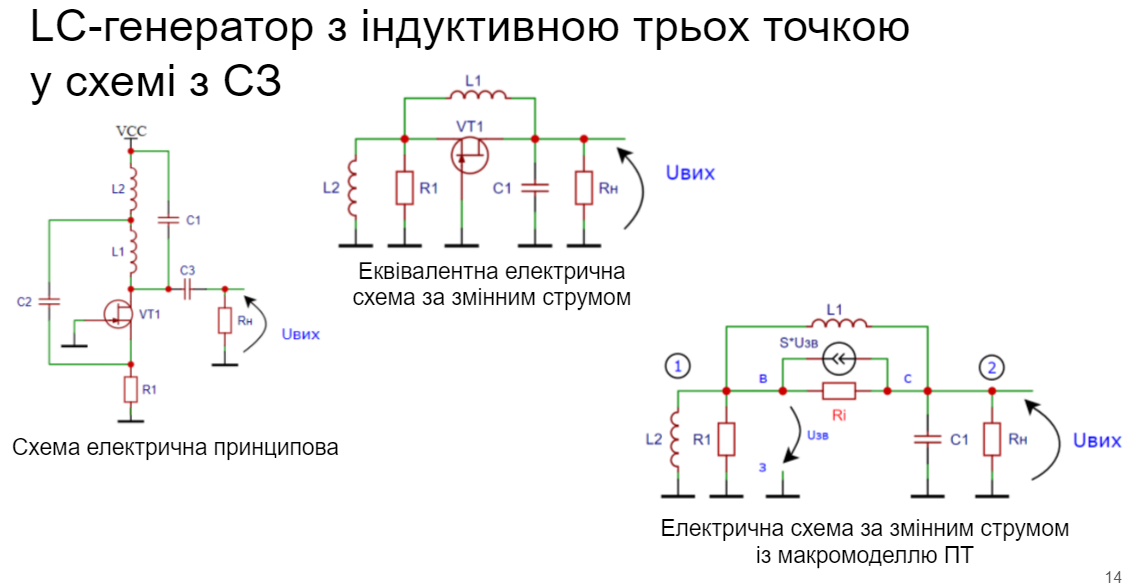
\includegraphics[width=0.5\linewidth]{68.1.png}
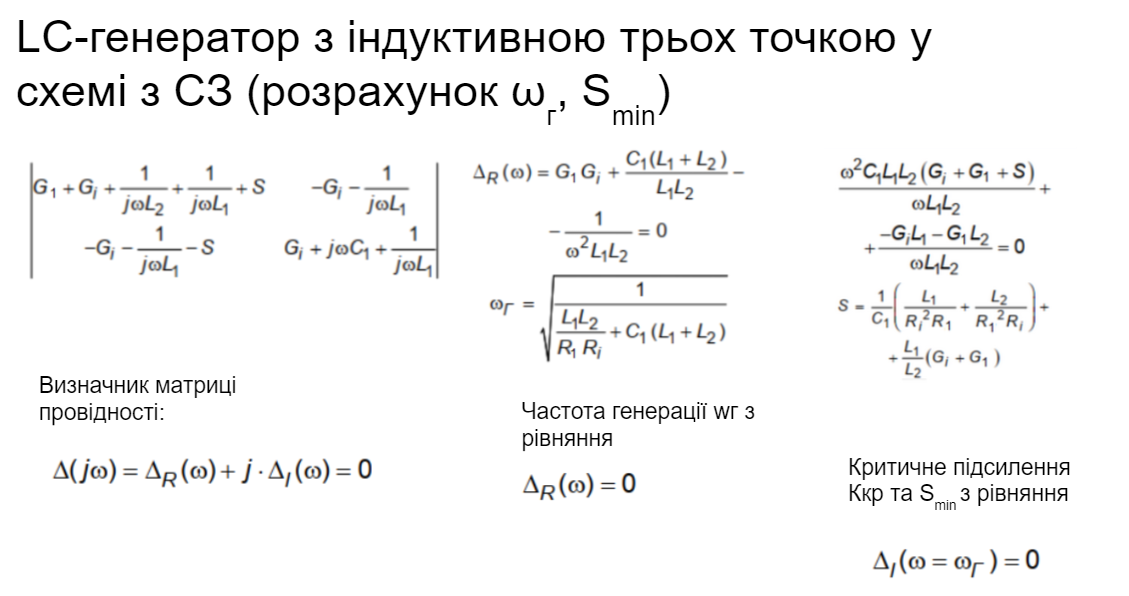
\includegraphics[width=0.5\linewidth]{68.2.png}

\hypertarget{35v}{\fbox{69}}\\[1cm]
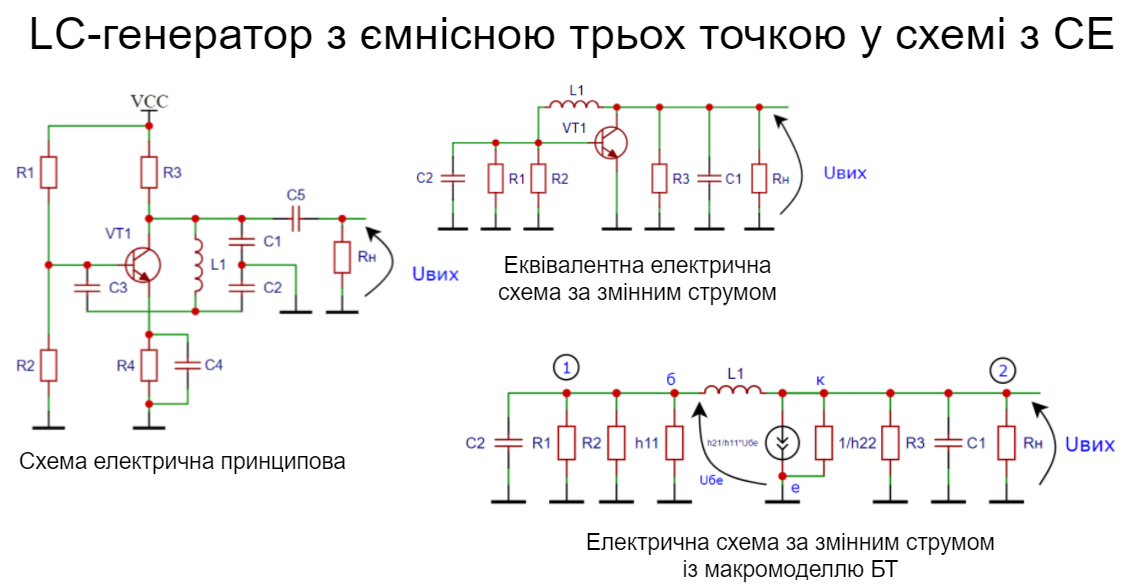
\includegraphics[width=0.5\linewidth]{69.1.png}
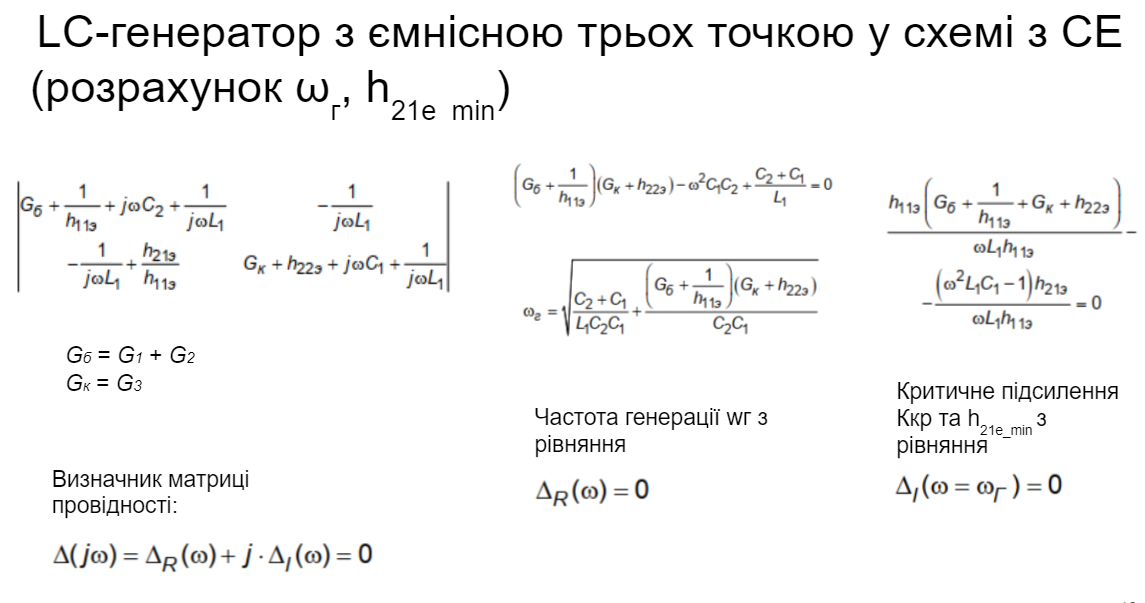
\includegraphics[width=0.5\linewidth]{69.2.png}

\hypertarget{36v}{\fbox{70}}\\[1cm]
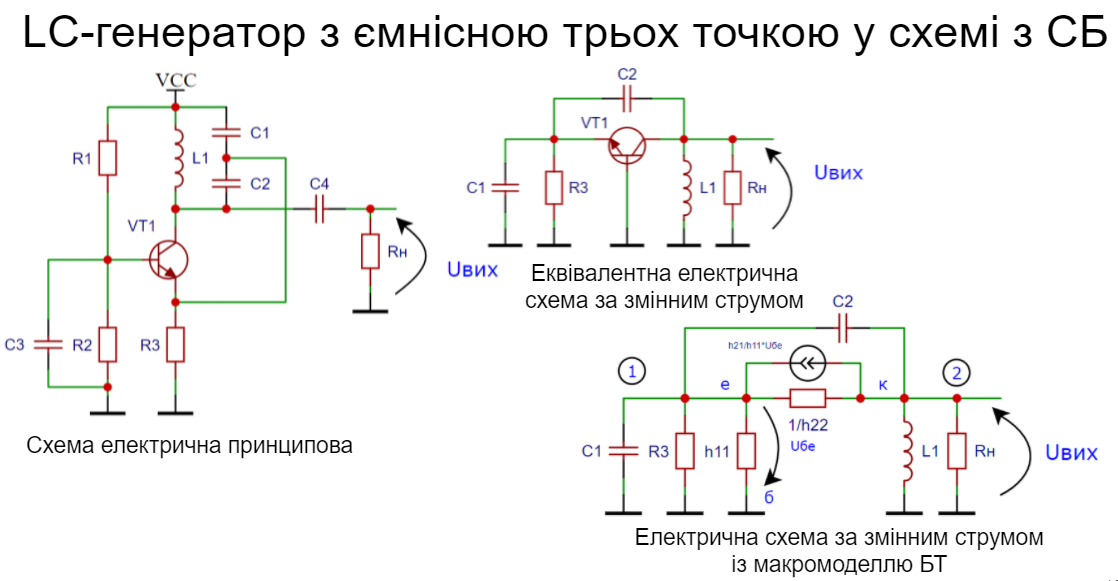
\includegraphics[width=0.5\linewidth]{70.1.png}
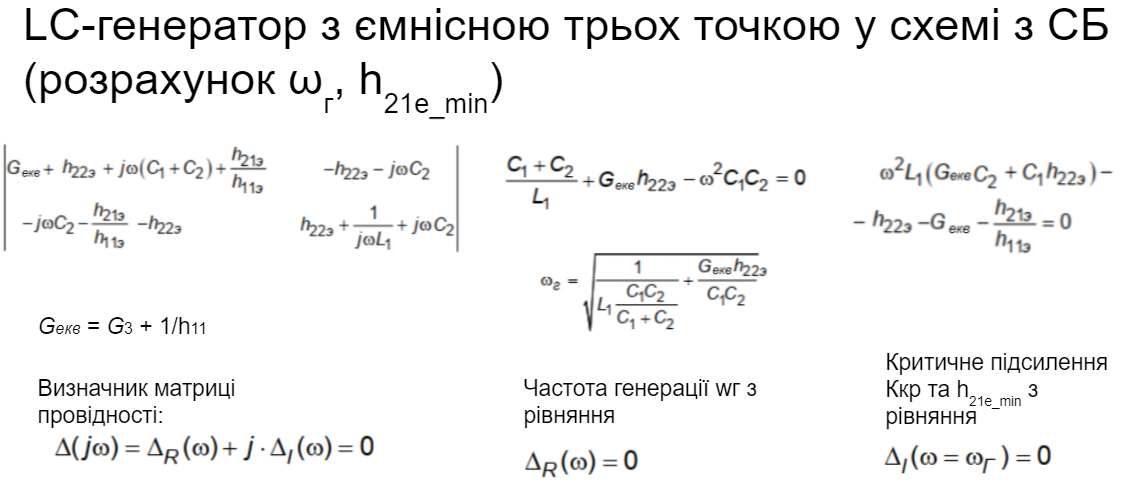
\includegraphics[width=0.5\linewidth]{70.2.png}

\hypertarget{37v}{\fbox{71}}\\[1cm]
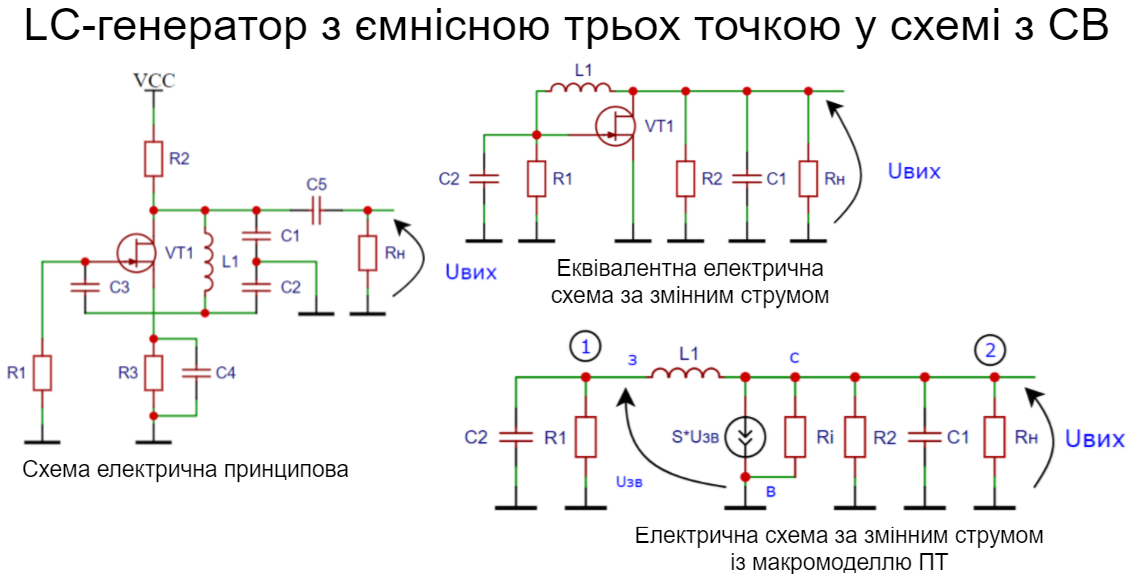
\includegraphics[width=0.5\linewidth]{71.1.png}
\includegraphics[width=0.5\linewidth]{71.2.png}

\hypertarget{38v}{\fbox{72}}\\[1cm]
\includegraphics[width=0.5\linewidth]{72.1.png}
\includegraphics[width=0.5\linewidth]{72.2.png}

\hypertarget{39v}{\fbox{73}}\\[1cm]
ой там короче лекция 14 сам если нужно прочитай там всё на игнлише я ебал  туда даже смотреть


\end{landscape}














\end{document}